\documentclass[12pt]{article}
\usepackage{graphicx,psfrag,amsfonts,float,mathbbol,xcolor,cleveref}
\usepackage{arydshln}
\usepackage{amsmath}
\usepackage{tikz}
\usepackage[mathscr]{euscript}
\usepackage{enumitem}
\usepackage{framed}
\usepackage{subcaption}
\usepackage{mathtools}
\usepackage{IEEEtrantools}
\usepackage{amsthm}
\usepackage[letterpaper, left=1in, top=1in, right=1in, bottom=1in,nohead,includefoot, verbose, ignoremp]{geometry}
\newcommand{\comment}[1]{\text{\phantom{(#1)}} \tag{#1}}
\newcommand\numberthis{\addtocounter{equation}{1}\tag{\theequation}}
\newcommand*\needsparaphrased{\color{red}}
\newcommand*\needscited{\color{orange}}
\newcommand*\needsproof{\color{blue}}
\newcommand*\outlineskeleton{\color{green}}
\newcommand{\PP}{\mathcal{P}}
\newcommand{\bfeps}{\mbox{\boldmath $\epsilon$}}
\newcommand{\bfgamma}{\mbox{\boldmath $\gamma$}}
\newcommand{\bflam}{\mbox{\boldmath $\lambda$}}
\newcommand{\bfphi}{\mbox{\boldmath $\phi$}}
\newcommand{\bfsigma}{\mbox{\boldmath $\sigma$}}
\newcommand{\bfbeta}{\mbox{\boldmath $\beta$}}
\newcommand{\bfalpha}{\mbox{\boldmath $\alpha$}}
\newcommand{\bfe}{\mbox{\boldmath $e$}}
\newcommand{\bff}{\mbox{\boldmath $f$}}
\newcommand{\bfone}{\mbox{\boldmath $1$}}
\newcommand{\bft}{\mbox{\boldmath $t$}}
\newcommand{\bfo}{\mbox{\boldmath $0$}}
\newcommand{\bfO}{\mbox{\boldmath $O$}}
\newcommand{\bfx}{\mbox{\boldmath $x$}}
\newcommand{\bfX}{\mbox{\boldmath $X$}}
\newcommand{\bfz}{\mbox{\boldmath $z$}}


\newcommand{\bfm}{\mbox{\boldmath $m}}
\newcommand{\bfy}{\mbox{\boldmath $y$}}
\newcommand{\bfd}{\mbox{\boldmath $d$}}
\newcommand{\bfc}{\mbox{\boldmath $c$}}
\newcommand{\bfa}{\mbox{\boldmath $a$}}
\newcommand{\bfb}{\mbox{\boldmath $b$}}
\newcommand{\bfY}{\mbox{\boldmath $Y$}}
\newcommand{\bfS}{\mbox{\boldmath $S$}}
\newcommand{\bfZ}{\mbox{\boldmath $Z$}}
\newcommand{\cardT}{\vert \mathcal{T} \vert}
%\newenvironment{theorem}[1][Theorem]{\begin{trivlist}
%\item[\hskip \labelsep {\bfseries #1}]}{\end{trivlist}}
%\newenvironment{corollary}[1][Corollary]{\begin{trivlist}
%\item[\hskip \labelsep {\bfseries #1}]}{\end{trivlist}}
%\newenvironment{proposition}[1][Proposition]{\begin{trivlist}
%\item[\hskip \labelsep {\bfseries #1}]}{\end{trivlist}}
%\newenvironment{definition}[1][Definition]{\begin{trivlist}
%\item[\hskip \labelsep {\bfseries #1}]}{\end{trivlist}}

\newtheorem{theorem}{Theorem}[section]
\newtheorem{lemma}[theorem]{Lemma}
\newtheorem{proposition}[theorem]{Proposition}
\newtheorem{corollary}[theorem]{Corollary}

\theoremstyle{definition}
\newtheorem{definition}{Definition}[section]
\newtheorem{example}{Example}[section]
\def\bL{\mathbf{L}}


\makeatletter
\renewcommand{\theenumi}{\Roman{enumi}}
\renewcommand{\labelenumi}{\theenumi.}
\renewcommand{\theenumii}{\Alph{enumii}}
\renewcommand{\labelenumii}{\theenumii.}
\renewcommand{\p@enumii}{\theenumi.}
\makeatother

 \begin{document}

\nocite{*}

Chapter 3 outlines a cohesive nonparametric approach to modeling $\phi\left(s,t\right)$ as a smooth bivariate function via P-splines, or penalized B-spline basis expansions. Eilers and Marx were the first to propose the method, which generalizes the work of O'Sullivan, which utilized derivative-based penalties to achieve smoothness in the fitted function. Their approach stands on two fundamental building blocks: B-splines and difference penalties. In the sections to follow, we will review the definition of the B-spline basis and derive the essential properties necessary for motivating the application of difference penalties on the spline coefficients. We will show that the simple difference penalties are easy to compute and achieve nearly the same construction as when utilizing the more computationally demanding derivative-based penalties, and demonstrate the effect of the roughness measure on the estimated functional coefficients.  


\section{A representation for piecewise polynomial functions}

Let $\xi = \left\{ \xi_1<\xi_2<\dots<\xi_{l+1} \right\}$ be a set of strictly increasing series of points, and let $k$ be a positive integer. Further, let $P_1,\dots,P_l$ denote a sequence of $l$ polynomials of order $k$. Then the correponding piecewise polynomial (pp) function of order $k$ is defined as follows:

\[
f\left(x\right) = P_i\left(x\right) \; \textup{if } \xi_i < x < \xi_{i+1}
\] 
\noindent
for $i=1,\dots,l$. $\left\{\xi\right\}$ are known as the breakpoints of $f$. At the interior breakpoints, $\xi_2,\dots, \xi_l$, the function value is defined by specifying $f$ to be right continuous; that is, 
\[
f\left(\xi_i\right) = f\left(\xi_i^+\right),\quad i=2,\dots,l
\]
However, in a sense, without this specification, the function has two values at any interior breakpoint: the value it gets from the polynomial piece to the left of the breakpoint, $f\left(\xi_i^-\right) = P_{i-1}\left(\xi_i\right)$, in addition to the value it gets from the polynomial piece to the right of the breakpoint, $f\left(\xi_i^+\right) = P_{i}\left(\xi_i\right)$. To properly define the function, one can specify $f$ to be right-continuous:
\begin{equation}
f\left(\xi_i\right) \equiv f\left(\xi_i^+\right) 
\end{equation}

Denote the set of pp functions of order $k$ with breakpoints $\xi=\left\{\xi_1,\dots,\xi_{l+1}\right\}$ by 
\[
\mathcal{P}_{k,\xi}.
\]

$\mathcal{P}_{k,\xi}$ is a linear space having dimension $kl$, as it consists of $l$ polynomials, each having $k$ polynomial coefficients. The $j^{th}$ derivative of a pp $f$,
\[
D^jf
\]
\noindent
is a pp function of order $k-j$ having the same breakpoint sequence and constructed from the same $j^{th}$ derivatives of the polynomial pieces from which $f$ was constructed. This ``definition'' dodges much of the complicated discussion of the derivatives of a pp function at its breakpoints and thus must be treated with considerable care in context of the fundamental theorem of calculus.

\begin{proposition} \label{proposition:continuous_function}
A pp function, $f$ satisfies
\[
f\left(x\right) - f\left(a\right) = \int_a^x \left(Df\right)\left(t\right)dt\quad \textup{for all} \quad x
\]
if and only if $f$ is a continuous function.
\end{proposition}

Consider a piecewise constant function $f$: by the previous definition, its first derivative is identically zero, and is therefore equal to the usual derivative of $f$ if and only if $f$ is constant. The following definition gives the information necessary for a convenient and efficient representation of this class of functions:

\begin{definition}\label{definition:pp_representation}
The \emph{piecewise polynomial (pp) representation} of a function $f \in \PP_{k,\xi}$ consists of 
\begin{enumerate}
\item integers $k$ and $l$, specifying the order and number of polynomial pieces, respectively,
\item a strictly increasing set of breakpoints, $\xi_1,\xi_2,\dots, \xi_{l+1}$,
\item and the set of values of the right derivatives at each of the breakpoints, 
\[
c_{ij} = D^{j}f\left(\xi_i^+\right), \quad j=1,\dots,k;\quad i=1,\dots,l 
\]
\end{enumerate}
\end{definition} 
 
 \section{The truncated power basis and the spaces $\PP_{k,\xi,\nu}$}
This prerequisite information is merely for the ability to responsibly refer to the set of piecewise polynomial functions and have a shorthand way of doing so. These means enable us to introduce two sets of basis functions: first, the truncated power basis, followed by B-spline basis functions. We will see that both are closely related, with the former having some properties which leave them unattractive for function approximation and thus present the construction of B-splines and how to use them to construct a representation of $\mathcal{P}_{k}$. In practice, one typically is given some information about an unknown function, $g$, and the task is to construct a function $f \in \PP_{k, \xi}$ which satisfies conditions that $g$ also satisfies, and in addition, has a certain number of continuous derivatives. These conditions define a subspace of $\PP_{k,\xi}$, $\PP_{k,\xi, \nu}$ for which we will need a corresponding basis.


\subsection{Example: histogram smoothing by parabolic splines}
For illustrative purposes, consider the task of smoothing a histogram using parabolic splines. Suppose we are given points
\[
\tau_1 < \tau_2 < \dots < \tau_{n+1}
\]
and non-negative numbers $h_1, h_2, \dots, h_n$, with $h_i$ denoting the height of the histogram over the interval $\left(\tau_i, \tau_{i+1} \right)$. The histogram is an approximate representation of some underlying density function, $g$. Letting $\Delta \tau_i = \tau_{i+1}-\tau_i$, one may interpret $h_i\Delta \tau_i$ as (approximately) equal to the integral of $g$ over $\left[\tau_i, \tau_{i+1} \right]$. One may impose the following interpolation conditions on our smooth function, $f$:
\begin{equation*} 
\int_{\tau_i}^{\tau_{i+1}} f\left(x\right)dx = h_i\Delta \tau_i
\end{equation*} 
\noindent
for $i=1,\dots, n$. Let $f$ be a piecewise polynomial of order 3 having continuous first derivative:
\[
f \in \PP_{3,\xi} \cap \mathcal{C}^{\left(1\right)}
\]
Choose the breakpoint sequence $\xi$ to coincide with $\tau = \left\{\tau_1,\dots, \tau_{n+1} \right\}$. If $g$ is smooth and vanishes outside its support, $\left[ \tau_1,\tau_{n+1} \right]$, then
\[
g^{\left( j \right)}\left(\tau_1\right) = g^{\left( j \right)}\left(\tau_{n+1}\right) = 0,
\]
\noindent
for $j=0,1,\dots,d$, where $d$ characterizes the extent of the smoothness of $g$, we may also wish to require $f$ to obey two additional interpolation constraints:
\[
f\left( \tau_1 \right) = f\left( \tau_{n+1} \right) = 0,
\]
giving a total of $n+2$ interpolation conditions. These, along with the $2\left(n-1\right)$ continuity conditions yield a total $3n$ constraints on the $3n$ polynomial coefficients,
\[
c_{ji} \equiv D^{j-1} f\left(\xi_i^+ \right).
\]
These conditions lead to the system of equations:

\begin{align*}
c_{11} &  &  &  &  &  &  & & & & & & & &&&&= & 0  \\
c_{11} & \;+\;  & c_{21} \frac{\Delta\tau_{1}}{2!} & \;+\;   & c_{31} \frac{\left(\Delta\tau_{1}\right)^2} {3!}  & 			   & 		 		        &  	      & & & && & &&&& = & h_1\\
c_{11} & \; +\; & c_{21}\Delta\tau_{1}                 & \; + \; & c_{31}\frac{2\left(\Delta\tau_{1}\right)^2}{3!}  & \;-\; & c_{12} &  		        & 	      & & & & & &&&& = & 0\\
\vdots   &  		   & c_{21}  				     & \; + \; & c_{31} \Delta\tau_{1}  				     &  		   &  		 & \;-\;  & c_{22} & && & & &&&& = & 0\\
	   &  			   &             				     &                        & 								     &  		   &   c_{12} &\;+\; &  c_{22}\frac{\Delta\tau_2}{2} &\;+\; & c_{32}\frac{\left(\Delta\tau_2\right)^2}{3!} & & & & &&& = & h_2\\
	   &  			   &             				     &                        & 								     &  		   &   c_{12} &\;+\; &  c_{22}\Delta\tau_2        &\;+\; & c_{32}\frac{\left(\Delta\tau_2\right)^2}{2} & & &\dots &&&&  = & 0\\
	   	   &  			   &             				     &                        & 								     &  		   &   		 &	&  c_{22}        &\;+\; & c_{32}\Delta\tau_2 & & & \dots &&&&  = & 0\\
    &  &  &  &  &  &  & & & & && & &&&&  &\\
   &  &  &  &  &  &  & & & & && & &\ddots &&&  & \numberthis  \label{eq:histogram_smoothing_eqn_system}
\end{align*}

\subsection{The subspace, $\PP_{k,\xi,\nu}$}
One may quickly see that this system is two-thirds homogeneous; that is, for every integral interpolation constraint, we have two continuity constraints that lead to zeros on the right hand side of the equality. To solve \ref{eq:histogram_smoothing_eqn_system}, the homogeneous equations are solved, leaving a reduced set of equations. To do this, one may construct a set of linearly independent functions $\phi_1, \phi_2, \dots$ of the same size as the number of interpolation constraints which satisfy the homogeneous equations in \ref{eq:histogram_smoothing_eqn_system}. The smoother, $f$, is then constructed within this subspace of $\PP_{3,\xi}$ and has form 
\[
f = \sum_{j} \alpha_j \phi_j.
\] 

\noindent
The $\left\{ \phi_j \right\}$ span a particular subspace of $\mathcal{P}_{k, \xi}$, which is comprised of functions which satisfy the homogeneous equations in \ref{eq:histogram_smoothing_eqn_system}. In general, we may characterize these homogeneous equations in terms of a given function having a particular number of continuous derivatives, which may be expressed as follows:
\begin{eqnarray}
\mathscr{J}_{ij}f = 0, \quad  i&=&2,\dots,l \label{eq:tpf_linear_operator_penalty} \\
 j&=&1,\dots,\nu_i \nonumber
\end{eqnarray}
\noindent
where
\begin{equation}
\mathscr{J}_{ij}f = \lim_{x\rightarrow \xi^+} D^{j-1}f\left(x\right) - \lim_{x\rightarrow \xi^-} D^{j-1}f\left(x\right)
\end{equation}
\noindent
and $\nu = \left(\nu_1,\dots, \nu_l\right)$ is a vector of non-negative integers. Each $\nu_i$ specifies the number of continuity conditions impose on the function at the $i^{th}$ breakpoint, $\xi$, and $\mathscr{J}_{ij}$ is simply the size of the jump in the $\left(j-1\right)^{st}$ derivative at $\xi$.


\subsection{The truncated power functions}
As homogeneous conditions specified in \ref{eq:tpf_linear_operator_penalty} are done so in terms of a linear operator applied to the functions in the space, those functions $\left\{ g \in \PP_{k,\xi} \right\}$ constitute a linear subspace, denoted
\[
 \PP_{k,\xi, \nu} 
\]
\noindent
Now that the subspace is defined, we need a basis for it. One such candidate set of basis functions is the truncated power basis. Define

\[
\left(x-t\right)_+ = \max\left(0,x-t\right)
\]
\noindent
We may then define the truncated power function as follows:
\begin{align}
\begin{split}
\left(x-t\right)_+^p &= \left( \left(x-t\right)_+\right)^p\\
&= \left\{\begin{array}{lr}
	\left(x-t\right)^p, & x \ge t\\
	0 & x < t
	\end{array} \right.
	\end{split}
\end{align}

The function $g\left(x\right) = \left(\right)_+^p$ is a piecewise polynomial with a single breakpoint at $\xi$, and is continuous at this breakpoint for $p>0$. For $p=0$, it has a jump of size 1 at $\xi$. Since

\[
D\left( \cdot - \xi\right)_+^p = p \left( \cdot - \xi\right)_+^{p-1},
\]
\noindent
it is clear that $g$ has $p-1$ continuous derivatives. Define the set of linear operators $\left\{ \lambda_{ij} \right\}$ and corresponding functions $\left\{ \phi_{ij} \right\}$ as follows:

\begin{align}
\begin{split}
\lambda_{ij}f  &= \left\{\begin{array}{lr}
	 D^{j}f\left(\xi \right) & i=1\\
	D^{j}f\left(\xi^+ \right) -  D^{j}f\left(\xi^-\right) & i=2,\dots,l
	\end{array} \right. \\
\phi_{ij}\left(x\right) &= \left\{\begin{array}{lr}
	\frac{\left(x-\xi_i \right)^p}{j!} & i=1\\
	\frac{\left(x-\xi_i \right)_+^p}{j!} & i=2,\dots,l
	\end{array} \right. 	
	\end{split} \label{eq:PP_basis_decomposition_componenents}
\end{align}
\noindent for $j=0,\dots,k-1$. Per this definition, we have that $\phi_{ij} \in \PP_{k,\xi}$ for each $i=1,\dots,l$. Further, we have that 

\begin{align*}
\lambda_{ij}\phi_{pq} = \left\{\begin{array}{lr}
	1  & i=p,\;j=q\\
	0 & \textup{otherwise}
	\end{array} \right. ,
\end{align*}
\noindent
making $\left\{ \phi_{ij} \right\}$ a set of $kl$ linearly independent functions, and since $\PP_{k,\xi}$ has dimension $kl$, they constitute a basis for the space. We may represent any $g \in \PP_{k,\xi}$ in the form

\begin{equation*}
g = \sum_{i,j} \left(\lambda_{ij}g\right)\phi_{ij}
\end{equation*}
\noindent
Rewriting this expansion in the terms presented in \ref{eq:PP_basis_decomposition_componenents}, we have that we may express any function in the space as
\begin{equation} \label{eq:tpf_basis_expansion}
g\left(x\right) = \sum_{j=0}^{k-1} \left[ D^j g\left(\xi_1\right)\frac{\left(x-\xi_1\right)^j}{j!} + \sum_{i=2}^l \left[ D^j g\left(\xi_i^+\right)-D^j g\left(\xi_i^-\right) \right]\frac{\left(x-\xi_i\right)_+^j}{j!} \right]
\end{equation}

From this representation of the function, one can see that the coefficients of the basis functions are explicitly defined in terms of jumps of various derivatives of $g$ at the breakpoints. Thus, enforcing the homogeneous constraints 
\[
\mathscr{J}_{ij}f = 0, \quad i=2,\dots, l;\quad j=1,\dots,\nu_i
\]
is accomplished simply by restricting our attention to functions of the form \ref{eq:tpf_basis_expansion} for which these coefficients are zero. This implies that the reduced set of basis functions $\left\{ \phi_{ij} \right\}$, $i=1,\dots,l$, $j=\nu_{i},\dots,k-1$ is a basis for the subspace, $\PP_{k,\xi,\nu}$. (We let $\nu_1 =0$.) Then, every function $g^* \in \PP_{k,\xi}$ in satisfying the homogeneous equations may be written in exactly one way of the form
\begin{equation} \label{eq:tpf_subspace_basis_expansion}
g^* = \sum_{i=1}^l \sum_{j={\nu_i}}^{k-1} \alpha_{ij} \phi_{ij}
\end{equation}

\subsubsection{The pitfalls of the truncated power basis}

While the truncated power basis initially appears quite attractive for smoothing problems involving piecewise polynomials, they exhibit properties that can lead to poor function representations. In order to discuss these characteristics, we must first introduce the notion of the \emph{condition} of a function representation.

\begin{definition}\label{definition:basis_condition}
Consider a piecewise polynomial representation of a function, $p$:
\begin{equation} \label{eq:polynomial_representation}
p = \sum_{i=1}^n a_i P_i
\end{equation}
\noindent
where $a = \left(a_1,\dots,a_n\right)$ is a coefficient vector and $\left\{ P_i\right\}$ is a set of polynomial functions defined on a closed interval $\left[a,b\right]$. We define the \emph{size} of the polynomial $p$ to be
\[
\left \lVert p \right \rVert = \max_{a\le x\le b} \left \lvert p\left(x\right) \right \rvert,
\]
\noindent
and similarly, we define the size of the coefficient vector $a$ to be
\[
\left \lVert a \right \rVert = \max_{1\le i \le n} \left \lvert a_i \right \rvert,
\]
Then, we can bound the size of the function $p$:
\begin{equation} \label{eq:polynomial_expansion_size_bounds}
m\left \lVert a \right \rVert \le \left \lVert \sum_{i=1}^n a_i P_i \right \rVert \le  M \left \lVert a \right \rVert
\end{equation}
\noindent
where 
\begin{align*}
m &= \min_a \frac{\left \lVert \sum_{i=1}^n a_i P_i \right \rVert}{\left \lVert a \right \rVert},\quad \textup{and}\\
M &= \min_a \frac{\left \lVert \sum_{i=1}^n a_i P_i \right \rVert}{\left \lVert a \right \rVert}
\end{align*}
The \emph{condition} of the representation of $p$ as written in \ref{eq:polynomial_representation} is given by 
\[
\textit{condition}\left( P_i \right) = \frac{M}{m}
\]
\end{definition}

The condition of a function representation quantifies the extent to which a slight change in the coefficient vector will impact the function itself. To see this, rather than the coefficient vector $a$, consider instead a perturbation of $a$:
\[
a + \delta a
\]
\noindent
The corresponding perturbed polynomial is given by 
\[
p + \delta p = \sum_{i=1}^n \left(a_i + \delta a_i \right) P_i
\]
By \ref{eq:polynomial_expansion_size_bounds}, we then have that 
\begin{equation*}
\frac{m\left \lVert \delta a \right \rVert}{M\left \lVert a \right \rVert} \le \frac{\left \lVert \delta p \right \rVert}{\left \lVert p \right \rVert} \le \frac{M\left \lVert \delta a \right \rVert}{m\left \lVert a \right \rVert},
\end{equation*}
\noindent
implying that a relative change of $\frac{\left \lVert \delta a \right \rVert}{\left \lVert a \right \rVert}$ to the coefficient vector may result in a relative change to the function $p$ as large as $\frac{M}{m} = \textit{condition}\left(P_i\right)$ times the relative change in $a$ (and at least as large as $\textit{condition}\left(P_i\right)^{-1}$). Note that the width of the interval 
\[
\left[\textit{condition}\left(P_i\right)^{-1}\frac{\left \lVert \delta a \right \rVert}{\left \lVert a \right \rVert},\textit{condition}\left(P_i\right) \frac{\left \lVert \delta a \right \rVert}{\left \lVert a \right \rVert} \right]
\]
\noindent
is increasing in $\textit{condition}\left(P_i\right)$; so large values of the condition of a representation imply that small relative changes in their corresponding coefficients may result in much smaller or much larger relative changes in the function being represented.

When representing a function $f \in \PP_{k,\xi}$ as in \ref{eq:tpf_basis_expansion}, two issues of concern arise: first, if $l$ is large, the value of the function at a point $x$ can potentially rely on far more than just $k$ of the basis coefficients. Additionally, if the breakpoints $\xi$ are very irregularly spaced, then the truncated power basis can present poor condition, which, in turn, can result in poorly conditioned linear systems (like the specific example given by \ref{eq:histogram_smoothing_eqn_system}.) Consequently, small perturbations of the basis function coefficients result in disproportional changes in the function.
\begin{figure}[H] 
\begin{center}
\begin{tikzpicture}
\draw[->] (-1,0) -- (11,0);
\draw[->] (0,-1) -- (0,3.5);
\filldraw[black] (0.1,1.3) circle (2pt)  ;
\filldraw[black] (1.1,1.3) circle (2pt)  ;
\filldraw[black] (2.1,1.3) circle (2pt)  ;
\filldraw[black] (3.1,1.3) circle (2pt)  ;
\filldraw[black] (4.45,2.4) circle (2pt)  ;
\filldraw[black] (4.75,0.2) circle (2pt)  ;
\filldraw[black] (6.1,1.3) circle (2pt)  ;
\filldraw[black] (7.1,1.3) circle (2pt)  ;
\filldraw[black] (8.,1.3) circle (2pt)  ;
\filldraw[black] (9.1,1.3) circle (2pt)  ;
\filldraw[black] (10,1.3) circle (2pt)  ;

\draw (0.1,1.3) -- (3.1,1.3);
\draw (3.1,1.3) -- (4.45,2.4);
\draw (4.45,2.4) -- (4.75,0.2);
\draw (4.75,0.2) -- (6.1,1.3);
\draw (6.1,1.3) -- (10,1.3);
\draw (0.1,0) node[above,scale=0.6] {$\xi_{1}$};
\draw (1.1,0) node[above,scale=0.6] {$\xi_{2}$};
\draw (2.1,0) node[above,scale=0.6] {$\xi_{3}$};
\draw (3.1,0) node[above,scale=0.6] {$\xi_{4}$};

 \draw (4.45,-.38) -- (4.45,-.22); 
 \draw (4.75,-.38) -- (4.75,-.22); 
\draw (4.45,-.3) -- (4.75,-.3) ;
\draw (4.6,-0.3) node[below,scale=0.6,align=center] {h};

\draw (6.1,0) node[above,scale=0.6] {$\xi_{7}$};
\draw (7.1,0) node[above,scale=0.6] {$\xi_{8}$};
\draw (8.1,0) node[above,scale=0.6] {$\xi_{9}$};
\draw (9.1,0) node[above,scale=0.6] {$\xi_{10}$};
\draw (10,0) node[above,scale=0.6] {$\xi_{11}$};
\foreach \coo in {.1,1.1,...,3.1}
{
  \draw (\coo,-1.5pt) -- (\coo,1.5pt); 
  \draw (\coo,0) node[below,scale=0.6] {\coo};
}
 \draw (4.45,-1.5pt) -- (4.45,1.5pt);
  \draw (4.75,-1.5pt) -- (4.75,1.5pt);
\foreach \coo in {6.1,7.1,...,9.1}
{
  \draw (\coo,-1.5pt) -- (\coo,1.5pt);
  \draw (\coo,0) node[below,scale=0.65] {\coo};
}
 \draw (10,0) node[below,scale=0.65] {10};
\draw (10,-1.5pt) -- (10,1.5pt);
\draw (-1.5pt,0.2) -- (1.5pt,0.2);
\draw (-1.5pt,1.3) -- (1.5pt,1.3);
\draw (-1.5pt,2.4) -- (1.5pt,2.4);
\draw (0,0.2) node[left,scale=0.6] {0.2};
\draw (0,1.3) node[left,scale=0.6] {1.3};
\draw (0,2.4) node[left,scale=0.6] {2.4};
\end{tikzpicture} 
\caption{The linear system for the coefficients of the truncated power basis is ill-conditioned for the above piecewise linear function  and choice of breakpoints, $\xi_1,\dots, \xi_{11}$.} \label{fig:piecewise_linear_tpf_fail}
\end{center}
\end{figure}


\begin{example} \label{ex:tpf_fail}
Suppose we wish to construct a function $f \in \PP_{k=2,\xi} \cap \mathscr{C}^{\left(0\right)}$ satisfying $f\left(\xi_i \right)=1.3$ for $i=1,\dots,4,7,\dots,11$, $f\left(\xi_5\right)=2.4$, and $f\left(\xi_6\right)=0.2$ with breakpoints specified as pictured in Fig~\ref{fig:piecewise_linear_tpf_fail}. 


The function $f$ is piecewise linear, so that $f \in \PP_{2,\xi,\nu}$ with $\nu_i=1$, $i=1,\dots, 11$. Then, for $f$ is of the form
\[
f\left(x\right) = \alpha + \beta\left(x-\xi_1\right) + \sum_{i=2}^l\alpha_i\left(x-\xi_i\right)_+
\]
\noindent

one can show that, given the continuity and interpolation constraints, $\alpha = 1.3$, $\beta = f^\prime\left(\xi_1\right) = 0$,  $\alpha_i = 0$ for $i \not \in \left\{4,5,6,7\right\}$, and 
\[
\begin{bmatrix}
\alpha_4\\
\alpha_5\\
\alpha_6\\
\alpha_7\\
\end{bmatrix} =  \begin{bmatrix}
\frac{1.1}{\Delta\xi_4}\\
-\frac{2.2}{\Delta \xi_5} -\frac{1.1}{\Delta\xi_4}\\
\frac{1.1}{\Delta\xi_6} + \frac{2.2}{\Delta \xi_5}\\
-\frac{1.1}{\Delta\xi_6} 
\end{bmatrix} = \begin{bmatrix}
\frac{1.1}{\Delta\xi_4}\\
-\frac{2.2}{h} -\frac{1.1}{\Delta\xi_4}\\
\frac{1.1}{\Delta\xi_6} + \frac{2.2}{h}\\
-\frac{1.1}{\Delta\xi_6} 
\end{bmatrix}
\]

When $h = \Delta \xi_5 \rightarrow 0$, we have 
\begin{align*}
\left(x-\xi_5\right)_+ &\approx \left(x-\xi_6\right)_+\\
\alpha_5  &\approx -\alpha_6 >> 1,
\end{align*}
\noindent
leading to a loss of significance in the evaluation of the function. For example, if we were to choose $\xi_5=4.5$, $\xi_6=4.8$, making $h=0.3$, with five significant decimal digit arithmetic, then we get
\[
\alpha=1.30000,\; \beta= 0.00000,\;\alpha_4= 0.78571,\;\alpha_5= -8.11905,\;\alpha_6= 8.17949,\;\alpha_7= -0.84615
\]
and the other $\alpha_i=0$. Evaluating the corresponding function at $x=9.6$ yields $1.299987$ rather than the correct value of 1.3. This error becomes larger as $h$ approaches 0.
\end{example}

A quick remedy for the problem in \ref{ex:tpf_fail} is to replace the truncated power basis with the set of hat functions:

\[
H_i\left(x\right)=\left\{
\begin{array}{lr}
\left(x-\xi_i\right)/\Delta\xi_{i-1}, & \xi_{i-1} < x \le \xi_i\\
\left(\xi_{i+1}-x\right)/\Delta\xi_{i}, & \xi_{i} < x \le \xi_{i+1}\\
0 & otherwise
\end{array}  \right.
\]
\noindent
To utilize the hat functions, we augment $\xi_1,\dots,\xi_12$ with two additional breakpoints: $\xi_0 \le \xi_1$ and $\xi_{12} \ge \xi_{11}$. Then,

\begin{align*}
f\left(x\right) = 1.3H_1\left(x\right) + \dots + 1.3H_4\left(x\right) &+ 2.4H_5\left(x\right) \\
 &+   0.2H_6\left(x\right)+ 1.3H_7\left(x\right) + \dots + 1.3H_{11}\left(x\right)
\end{align*}

Even just using just two decimal digit arithmetic, we have $f\left(9.5\right) = 1.3$. Even as $h \rightarrow 0$, $f$ is well represented using the hat functions as a basis. More generally speaking, \emph{B-splines}, which are a generalization of these hat functions, overcome the issues that accompany the truncated power basis previously illustrated. The alternative basis is constructed by assembling linear combinations of the truncated power functions, forming a set of basis functions having ``small'' support: the functions vanish outside a small interval of their domain. In the following section, we will define the $k^{th}$-order B-splines as scaled \emph{divided differences} of truncated power functions. We will also show that every subspace $\PP_{k,\xi,\nu}$ has a basis consisting of these functions, bringing forth a B-spline representation of any pp function. 

\section{The B-spline representation of piecewise polynomial functions}

We will present an introduction to B-splines and their properties in the section to follow. As these basis functions are defined in terms of divided differences of the truncated power functions discussed in the previous section, we must first review the definition and properties of the divided difference operator. While there are many ways of defining divided differences, the following (somewhat nonconstructive definition) is intuitive and adequate for our purposes here.

\subsection{The divided difference}

\begin{definition}\label{definition:divided_difference}
The \emph{$k^{th}$ divided difference} of a function $g$ at the points $\tau_i,\dots,\tau_{i+k}$, denoted
\[
\left[ \tau_i,\dots,\tau_{i+k} \right]g,
\]
is the leading coefficient of the polynomial of order $k+1$ which \emph{agrees with $g$} at $\tau_i,\dots,\tau_{i+k}$.
\end{definition}
This leads us to the following definition:

\begin{definition}\label{definition:agrees_with_g}
Let $\left\{\tau_i \right\}_{i=1}^n$ denote a sequence of points. We say that a function $f$ \emph{agrees with} a function $g$ at $\tau$ if, for every point $\tau$ which occurs $m$ times in $\left\{\tau_i \right\}$, $f$ and $g$ agree up to $m$ derivatives at $\tau$; i.e.
\[
f^{\left(i-1\right)}\left(\tau\right) = g^{\left(i-1\right)}\left(\tau\right), \quad i=1,\dots,m
\]
\end{definition}

\subsubsection{Properties of the divided difference}
Definition~\ref{definition:divided_difference} yields the following properties of the $k^{th}$ divided difference:

\begin{enumerate} \label{dd_properties}
\item \label{eq:dd_property_1} Let $\left\{ p_i \right\}$, $i=1,2,\dots$ denote a sequence of polynomials with $p_i$ having order $i$. If $p_i$ agrees with a function $g$ at $\tau_1,\dots, \tau_i$ for $i=k,k+1$, then 
	\begin{equation*} 
	p_{k+1}\left(x\right) = p_k\left(x\right) + \left(x-\tau_1\right)\cdot \dots \cdot \left(x-\tau_k\right)\left[\tau_1,\dots,\tau_{k+1}\right]g
	\end{equation*}
	\begin{proof}
	Note that $p_{k+1}\left(x\right) - p_{k}\left(x\right)$ is a polynomial of order $k+1$ and vanishes at $\tau_1,\dots,\tau_k$, and, by definition, has $\left[\tau_1,\dots,\tau_{k+1}\right]g$ as its leading coefficient. Consequently, $p_{k+1}-p_k$ is of the form
	\begin{equation*}
	p_{k+1}\left(x\right) - p_{k}\left(x\right) = c\prod_{j=1}^k \left(x-\tau_j\right)
	\end{equation*}
	\noindent
	where 
	\[
	c = \left[\tau_1,\dots,\tau_{k+1}\right]g
	\]
	\end{proof}
	This tells the reader that interpolating polynomials may be constructed using divided differences by adding the interpolation points one by one, giving the \emph{Newton form} of the $n^{th}$ order polynomial which agrees with $g$ at $\tau_1,\dots,\tau_n$:
	\[
	p_n\left(x\right) = \sum_{i=1}^n \left(x-\tau_{1}\right)\times \dots \times \left(x-\tau_{i-1}\right) \left[\tau_1,\dots,\tau_{i-1} \right]g
	\]
\item \label{eq:dd_property_2} $\left[\tau_i,\dots,\tau_{i+k} \right]g$	is symmetric in its arguments $\tau_i,\dots, \tau_{i+k}$ (since the interpolating polynomial depends only on the points of interpolation and not the order in which they are specified.)
\item \label{eq:dd_property_3} $\left[\tau_i,\dots,\tau_{i+k} \right]g$ is a linear operator; if we let 
\[
f= \alpha g + \beta h
\]
\noindent
for some functions $g,h$ and scalars $\alpha, \beta$, then
\[
\left[\tau_i,\dots,\tau_{i+k} \right]f = \alpha\left[\tau_i,\dots,\tau_{i+k} \right]g + \beta\left[\tau_i,\dots,\tau_{i+k} \right]h
\]
\item \label{eq:dd_property_4} If $f=gh$, then
\[
\left[\tau_i,\dots,\tau_{i+k} \right]f  = \sum_{j=i}^{i+k} \left[\tau_i,\dots,\tau_{i+k} \right]g \left[\tau_i,\dots,\tau_{i+k} \right]h 
\]
\item \label{eq:dd_property_5} If $g$ is a polynomial of degree $\le k$, then $\left[\tau_i,\dot,\tau_{i+k}\right]g$ is constant as a function of $\tau_i,\dot,\tau_{i+k}$. In particular,
\[
\left[\tau_i,\dot,\tau_{i+k}\right]g = 0 \quad \forall g \in \PP_{k}
\]
The polynomial which agrees with $g$ at $\tau_i,\dots, \tau_{i+k}$ or any other $k+1$ points must be $g$ itself due to the uniqueness of interpolating polynomials. For more details, we refer the reader to {\needscited{A Practical Guide to Splines, DeBoor}}.
\item \label{eq:dd_property_6} $\left[\tau_i,\dots,\tau_{i+k} \right]g$ is a continuous function of its $k+1$ arguments in case $g\in \mathscr{C}^{\left(k\right)}$ (that is, if $g$ has $k$ continuous derivatives.)
\item \label{eq:dd_property_7} If $g\in \mathscr{C}^{\left(k\right)}$, then there exists a point $\xi$ in the smallest interval containing $\tau_i,\dots,\tau_{i+k}$ such that 
\[
\left[\tau_i,\dots,\tau_{i+k} \right]g = \frac{g^{\left(k\right)}\left(\xi\right)}{k!}
\] 
\item \label{eq:dd_property_8}\[
\left[\tau_i,\dots,\tau_{i+k} \right]g = \left\{\begin{array}{ll}
\frac{g^{\left(k\right)}\left(\tau_i\right)}{k!} & \tau_i= \dots = \tau_{i+k},\;\;g\in \mathscr{C}^{\left(k\right)} \\
\frac{\left[\tau_i,\dots,\tau_{r-1},\tau_{r+1},\dots,\tau_{i+k} \right]g-\left[\tau_i,\dots,\tau_{s-1},\tau_{s+1},\dots,\tau_{i+k} \right]g}{\tau_s-\tau_r} &  \tau_r,\tau_s \textup{ are any two distinct}\\
& \textup{  points in } \left\{\tau_i,\dots,\tau_{i+k}\right\}
\end{array} \right.
\]
\item \label{eq:dd_property_9} Let $\tau = \left\{\tau_i \right\}$, $i=1,\dots,n$ be a nondecreasing sequence, and let $g$ be a ``smooth enough'' function. Define the restriction of $g$ to the sequence $\tau$ to be the vector $g \vert_\tau = \left(g_1,\dots,g_n\right)^T$, where
\[
g_i = g^{\left(r\right)}\left(\tau_i\right),\quad r=\max\left\{j:\;\tau_{i-j}=\tau_i\right\}
\]
For any $1 \le r \le s \le n$, there exist constants $\left\{d_i \right\}$, $i=1,\dots,n$ which depend only on $r$, $s$, and $\tau$ and are free of $g$ such that 
\begin{equation} \label{eq:dd_property_9_punchline}
\left[\right]g = \sum_i=1^n d_i g_i
\end{equation}
\begin{proof}
The proof is done by induction on $s-r$. The statement is obvious for the case where $s-r=0$; all $d_i = 0$ except the constant corresponding to $g\left(\tau_r\right)$, which is equal to $1$. For any $r < s$, if $\tau_r= \dots = \tau_s$, then 
\[
\left[\tau_r,\dots, \tau_s\right]g = \frac{g^{\left(s-r\right)}\left(\tau_r\right)}{\left(s-r\right)!}
\]
so that \ref{eq:dd_property_9_punchline} holds with a single $d_j = \frac{1}{\left(s-r\right)!}$ and all other $d_i = 0$. The index $j \le s$ of the nonzero constant depends only on the number of $\tau_j$ with $j<r$ and $\tau_j = \tau_r$.

Assume that \ref{eq:dd_property_9_punchline} holds for $s-r < k$. Consider $s-r = k$ with $\tau_r < \tau_s$. By the induction hypothesis, there are coefficients $\left\{d_i^\prime\right \}$ and $\left\{d_i^{\prime\prime}\right\}$
\end{proof}
\end{enumerate}

In the following section, we will present B-splines as divided differences of the truncated power basis and present some of their properties which come as a result of the properties of the divided difference presented in this section.

\section{A B-spline representation for pp functions}

\begin{definition} \label{definition:order_k_Bspline}
Let $t= \left\{ t_i \right\}$ denote a non-decreasing sequence. The $i^{th}$ B-spline of order $k$ which corresponds to the knot sequence $t$ is defined by 
\begin{equation} \label{eq:bspline_definition}
B_{i,k,t}\left(x\right) = \left(t_{i+k}-t_i\right)\left[t_i,\dots,t_{i+k}\right]\left(\cdot -x\right)_+^{k-1}
\end{equation}
\end{definition}

The placeholder notation, $\left(\cdot - x\right)_+^{k-1}$, is used to indicate that the $k^{th}$ divided difference of the function $g\left(t \right) = \left(t-x\right)^{k-1}_+$ is obtained by fixing $x$ and applying the divided difference to $g\left(t \right)$ as a function of $t$ alone. Henceforth, we will write $B_i$ rather than $B_{i,k,t}$ when the spline order and knot sequence can be inferred from surrounding context.

\subsection{Properties of B-splines}

\begin{enumerate} \label{eq:BS_properties}
\item \label{eq:BS_property_1} $B_i\left(x\right)$ has isolated support:
\[
B_i\left(x\right) = 0, \quad x \not \in \left[t_{i},t_{i+k}\right]
\]
To see this, note that if $x \not \in \left[t_{i},t_{i+k}\right]$, then $g\left(t \right) = \left(t-x\right)^{k-1}_+$ is a polynomial of degree $< k$ on $\left[t_{i},t_{i+k}\right]$, thus by \ref{dd_properties} \ref{eq:dd_property_5},
\[
\left[t_{i},\dots,t_{i+k}\right]g = 0.
\]
As a result, for a set of B-splines of order $k$ corresponding to the knot sequence $t$, only $k$ of them are nonzero on $\left[t_{j},t_{j+k}\right]$: $B_{j-k+1},B_{j-k+2},\dots,B_{j}$.
\item \label{eq:BS_property_2} The $i^{th}$ B-spline of order is defined as the $k^{th}$ divided difference of $\left(\cdot - x\right)_+^{k-1}$ times a normalization factor: $\left(t_{i+k}-t_i\right)$. This normalization, using \ref{dd_properties} \ref{eq:dd_property_8}, allows us to write 
\begin{equation} \label{eq:BS_norm_rr}
B_i\left(x\right)=\left[t_{i+1},\dots,t_{i+k} \right]\left(\cdot - x\right)_+^{k-1} - \left[t_{i},\dots,t_{i+k-1} \right]\left(\cdot - x\right)_+^{k-1}
\end{equation}
For $x \in \left(t_{j},t_{j+1}\right)$, by \ref{dd_properties} \ref{eq:dd_property_1},
\begin{align}
\sum_{i} B_i\left(x\right) &=  \sum_{i=j+1-k}^{j} B_i\left(x\right) \nonumber\\
&= \sum_{i=j+1-k}^{j} \left[t_{i+1},\dots,t_{i+k} \right] \left(\cdot - x\right)_+^{k-1} - \sum_{i=j+1-k}^{j} \left[t_{i},\dots,t_{i+k-1} \right] \left(\cdot - x\right)_+^{k-1} \nonumber \\
&= \left[t_{j+1},\dots,t_{j+k} \right] \left(\cdot - x\right)_+^{k-1} - \left[t_{j+1-k},\dots,t_{j} \right] \left(\cdot - x\right)_+^{k-1} \nonumber \\
&= 1 - 0 \label{eq:unity_equality}
\end{align}
The last equality in \ref{eq:unity_equality} is a consequence of the following: for $x \in \left(t_j,t_{j+1}\right)$, $g\left(t\right)=\left(t - x\right)_+^{k-1}$ is a $k-1$ degree polynomial with unit leading coefficient on $\left[ t_{j+1},t_{j+k} \right]$, so by \ref{dd_properties} \ref{eq:dd_property_5}, 
\[
\left[ t_{j+1},\dots,t_{j+k} \right]g=1.
\]
On $\left[ t_{j+1-k},t_{j} \right]$, $g$ is identically $0$, hence $\left[ t_{j+1-k},\dots,t_{j} \right]g = 0$.   
\item \label{eq:BS_property_3}Each $B_i\left(x\right)$ is positive on its support. Applying Leibnitz's formula (\ref{dd_properties} \ref{eq:dd_property_4}) to the product
\[
\left[t_i,\dots,t_{i+k} \right]\left(t-x\right)_+^{k-1} = \left[t_i,\dots,t_{i+k} \right]\left(t-x\right) \left(t-x\right)_+^{k-2},
\] 
we have
\begin{align}
\left[t_i,\dots,t_{i+k} \right]\left(t-x\right)_+^{k-1} &=  \left[t_i,\dots,t_{i+k} \right]\left(t-x\right) \left(t-x\right)_+^{k-2} \nonumber\\
&= \sum_{r=i}^{i+k}\left[t_i,\dots,t_{i+r} \right] \left(t-x\right)\left[ t_r,\dots,t_{i+k}\right]\left(t-x\right)_+^{k-2} \nonumber \\
&= \bigg[ \left[t_i\right]\left(t-x \right) \bigg]\bigg[ \left[ t_i,\dots,t_{i+k}\right]\left(t-x\right)_+^{k-2}\ \bigg]\nonumber \\
& \qquad \qquad + \bigg[ \left[t_i,t_{i+1}\right]\left(t-x \right) \bigg]\bigg[ \left[ t_{i+1},\dots,t_{i+k}\right]\left(t-x\right)_+^{k-2} \bigg] \nonumber \\
&= \left(t_i-x \right) \left[ t_{i},\dots,t_{i+k}\right]\left(t-x\right)_+^{k-2} \nonumber \\
& \qquad \qquad \qquad \qquad \qquad +  1 \cdot \left[ t_{i+1},\dots,t_{i+k}\right]\left(t-x\right)_+^{k-2} \label{eq:nonneg_star}
\end{align}
since $\left[ t_i,\dots,t_j\right]\left(\cdot-x\right) = 0$ for $j>i+1$. By \ref{dd_properties} \ref{eq:dd_property_8}, 
\[
\left(t_i-x \right) \left[ t_{i},\dots,t_{i+k}\right]g = \frac{t_i-x}{t_{i+k}-t_{i}}\bigg[\left[ t_{i+1},\dots,t_{i+k}\right]g -\left[ t_{i},\dots,t_{i+k-1}\right]g   \bigg],
\]
and we may express \ref{eq:nonneg_star} as 
\begin{align*}
\left[ t_{i},\dots,t_{i+k}\right]\left(\cdot - x\right)^{k-1}_+ &= \frac{x-t_i}{t_{i+k}-t_{i}}\left[ t_{i},\dots,t_{i+k-1}\right] \left(\cdot-x\right)_+^{k-2}  \\
& \quad + \frac{t_{i+k}-x}{t_{i+k}-t_{i}}\left[ t_{i+1},\dots,t_{i+k}\right] \left(\cdot-x\right)_+^{k-2} 
\end{align*}
which we can write in terms of the normalized B-spline:
\begin{equation} \label{eq:nonneg_starstar}
\frac{B_{i,k}\left(x\right)}{t_{i+k}-t_i} = \frac{x-t_i}{t_{i+k}-t_{i}}\frac{B_{i,k-1}\left(x\right)}{t_{i+k-1}-t_i} + \frac{t_{i+k}-x}{t_{i+k}-t_{i}} \frac{B_{i+1,k-1}\left(x\right)}{t_{i+k}-t_{i+1}}
\end{equation}
This shows that we can write the $i^{th}$ B-spline of order $k$ as a convex combination of the $i^{th}$ and $\left(i+1\right)^{st}$ B-splines of order $k-1$ since 
\[
\frac{x-t_i}{t_{i+k}-t_{i}} + \frac{t_{i+k}-x}{t_{i+k}-t_{i}}  = 1,
\]
and each of these weights are positive for $t_i < x < t_{i+1}$. If
\[
\begin{array}{lr}
B_{j,k-1}\left(x\right) > 0, & t_j < x < t_{j+k-1} \; \textup{for all } j,
\end{array}
\]
then by \ref{eq:nonneg_starstar}, we have that 
\[
B_{i,k}\left(x\right) > 0,  \qquad t_i < x < t_{i+k}
\]
since $B_{j,k-1}= 0$ for $x \not \in \left[t_j,t_{j+k}\right]$ by \ref{eq:BS_properties} \ref{eq:BS_property_1} and by induction over $k$, starting with the fact that 
\[
B_j,1\left(x\right) = \left\{ \begin{array}{lr}
1 & t_j \le x < t_{j+1}\\
0 & otherwise
\end{array}\right.
\]
Properties \ref{eq:BS_property_1}, \ref{eq:BS_property_2}, and \ref{eq:BS_property_3} demonstrate that a sequence of B-splines form a \emph{partition of unity}: a set of non-negative functions which sum, pointwise, to one.
\end{enumerate}

\begin{example}
Figure~\ref{fig:deboor_bspline_basis} show fives parabolic B-splines corresponding to the set of knots $\left\{0,1,1,3,4,6,6,6 \right\}$. It is clear that each spline has compact support and is non-negative on this support. The function values are provided at select domain values so that property \ref{eq:BS_property_2} is evident, though it is worth noting that 
\[
\sum_{i=1}^6 B_i\left(x\right) = 1
\]
only on $\left[\frac{1}{6},1\right]$. In particular, they do not sum to 1 on $\left(0,\frac{1}{6}\right)$. 

Each $B_i$ is piecewise parabolic, with the breakpoints being locations of discontinuity of the function or one of its derivatives. $B_5$ is discontinuous at $x=6$, as the knot at 6 is repeated three times in the knot sequence defining $B_5$: $\left\{t_5,t_6,t_7,t_8\right\}$.

$B_1$, $B_2$, and $B_4$ have discontinuous first derivatives since 1 is repeated twice in the knots defining $B_1$ and $B_2$, and 6 is repeated twice in the knots defining $B_4$. The relationship between knot replication and smoothness will be discussed in more detail in the following section.

\begin{figure}[h]
 \begin{center}
 \graphicspath{{img/}}
  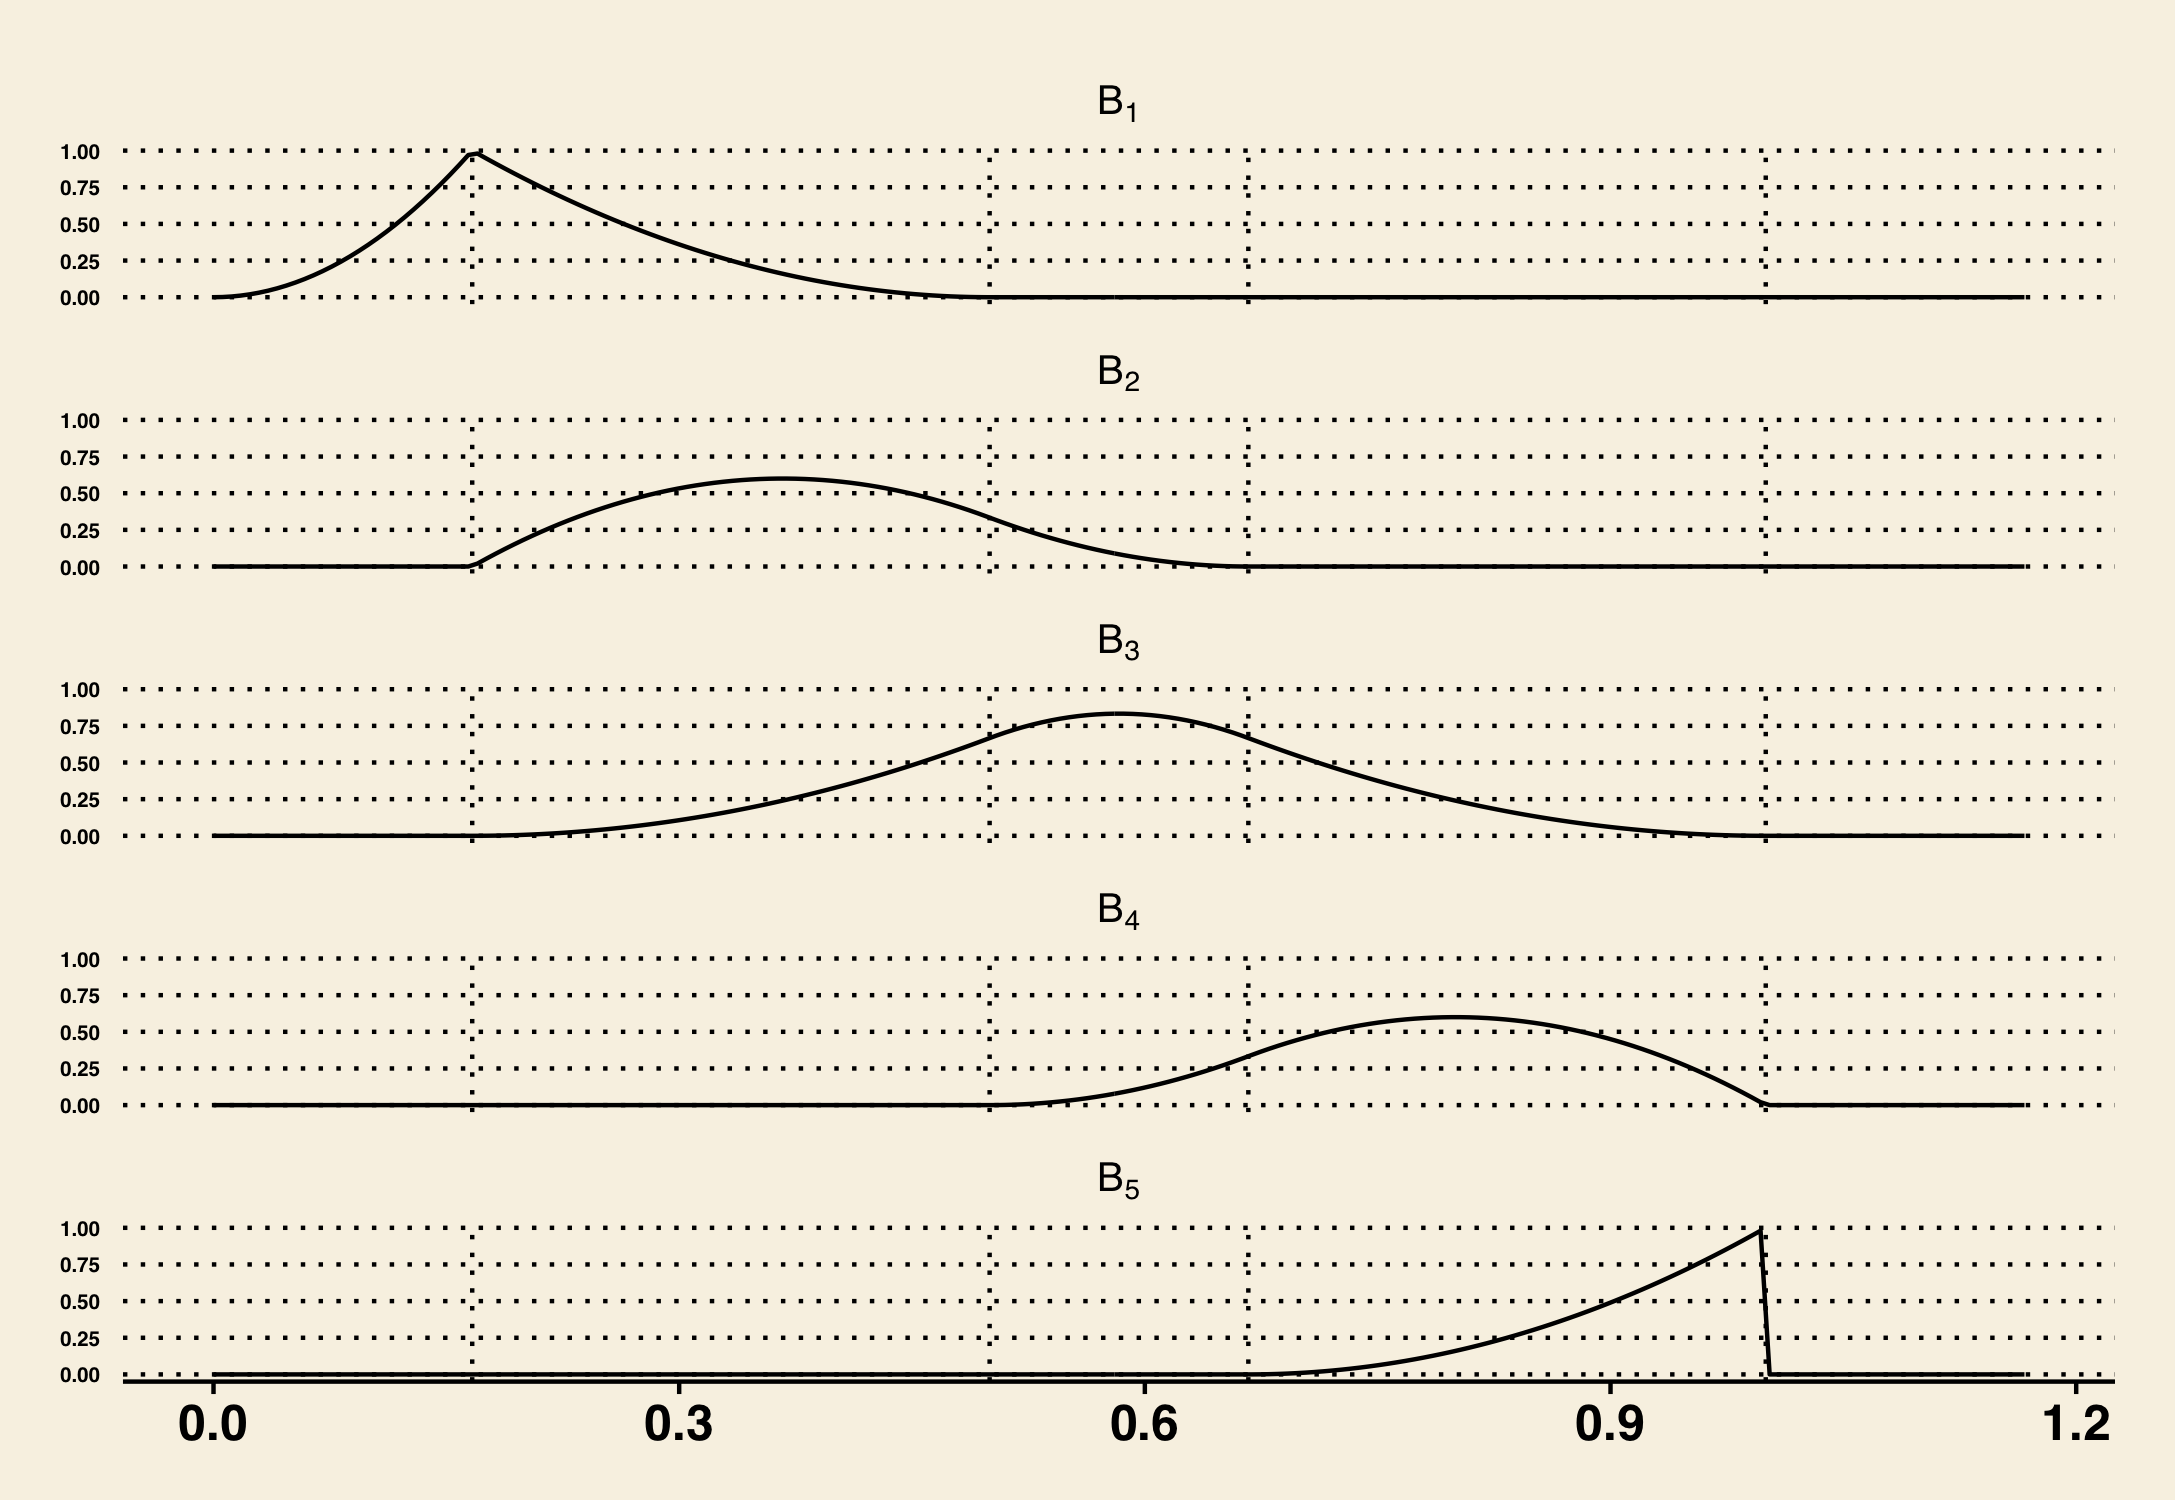
\includegraphics[width=7in, height=5in]{deboor_parabolic_bsplines.png}
  \caption{Parabolic B-splines corresponding to knot sequence $\{0,1,1,3,4,6,6,6\}$, illustrating the connection between knot multiplicity and smoothness.}\label{fig:deboor_bspline_basis}
\end{center}
\end{figure}
\end{example}

\subsubsection{The Curry-Schoenberg Theorem}

There is an extensive body of literature 
\begin{definition}
A \emph{spline function of order k with knot sequence t} is any linear combination of B-splines of order $k$ for the knot sequence $t$. We denote this set of functions by 
\[
\mathscr{S}_{k,t} = \bigg\{ \sum_i \alpha_i B_{i,k,t}: \quad \alpha_i \in \Re \bigg \}
\]
\end{definition}

\begin{theorem}{Curry-Schoenberg Theorem} \label{curryschoenbergthm}
For a strictly increasing sequence $\xi = \big\{ \xi_i \big\}$, $i=1,\dots, l+1$ and a sequence of non-negative integers $\nu = \big\{ \nu_j \big\}$, $j=2, \dots,l$ with $\nu_j \le k$ for all $j$, define
\begin{align*}
n &= k + \sum_{i=2}^l\left(k-\nu_i\right) = kl - \sum_{i=2}^l \nu_i \\
&= \textup{dim}\left(\PP_{k,\xi,\nu}\right)
\end{align*}
and let 
$t = \big\{ t_i \big\}$, $i=1, \dots,n+k$ be a non-decreasing sequence with 
\begin{enumerate}
\item \begin{align*}
 t_1 & \le t_2 \le  \dots \le t_{k} \le \xi_1\\
 \xi_{l+1} & \le t_{n+1} \le  \dots \le t_{n+k}\\
\end{align*}
\item $\xi_i$ occurs exactly $k-\nu_i$ times in $t$ for $i=2,\dots,l$.
\end{enumerate}
Then, the sequence of B-splines of order $k$ for the knot sequence $t$, $B_1,\dots, B_n$, is a basis for $\PP_{k,\xi,\nu}$ on the domain $\left[t_k,t_{n+1} \right]$. 
\end{theorem}

Theorem~\ref{curryschoenbergthm} gives an explicit prescription for the construction of a B-spline basis for any particular pp space, $\PP_{k,\xi,\nu}$, via the specification of $t$. These functions were named (B for `basis') for this theorem. The choice of $t$ controls the smoothness of the corresponding basis functions via knot multiplicities; the number of knots at a given breakpoint dictates the amount of smoothness at the breakpoint. Fewer knots placed at a breakpoint leads to more continuity conditions such that 
\[
\left[\mbox{\# continuity conditions at } \xi\right] + \left[\mbox{\# knots at } \xi\right] = k
\]
A knot with multiplicity $k$ yields a basis with no continuity conditions at that point, and a point where there are no knots forces $k$ continuity conditions there.

\subsubsection{The Curry-Schoenberg Proof}

\begin{proof}
We begin by showing that $B_i \in \PP_{k,\xi,\nu}$ for all $i$ as functions defined on $\left[t_k,t_{n+1}\right]$. Each $B_i = B_{i,k,t}$ is defined as the $k^{th}$ divided difference of $\left(t-x\right)_+^{k-1}$ at $t_i,\dots,t_{i+k}$ times a scalar, so by \ref{dd_properties} \ref{eq:dd_property_9}, we can find coefficients $d_i,\dots,d_{i+k}$ which depend only on $t_{i},\dots,t_{i+k}$ so that for any smooth function $g$, 
\begin{equation} \label{eq:cs_proof_star}
\left[t_i,\dots,t_{i+k} \right]g = \sum_{r=i}^{i+k} d_r g^{\left(j_r\right)}\left(t_r\right)
\end{equation}
with 
\[
j_r = \max \bigg\{s:\;\;r-s \ge i \mbox{ and } t_{r-s} = t_r;\;\;r=i,\dots,i+k\bigg\}.
\]
Using this, we may write 
\begin{equation} \label{eq:cs_proof_starstar}
B_i\left(x\right) = \left(t_{i+k}-t_i\right)\sum_{r=i}^{i+k} d_r \left(t_r - x\right)_+^{k-j_r-1}\frac{\left(k-1\right)!}{\left(k-j_r-1\right)!}.
\end{equation}
From \ref{eq:cs_proof_starstar}, it follows immediately that $B_i$ is a pp function of order $k$ with breakpoints $t_i,\dots,t_{i+k}$ (and consequently some of the $\left\{\xi_i\right\}$.)

Now, we must establish the number of continuous derivatives of each $B_i$ at each of its breakpoints, $\xi_i$, $i=2,\dots,l$. For any $B_i$, there cannot be a jump in its $s^{th}$ derivative across $\xi_j$ unless 
\[
\xi_j = t_r \mbox{ and } k-1-j_r = s
\]
for some $r \in \left\{ i,\dots,i+k \right\}$. Since 
\[
j_r = \# \;\; t_r = t_m \;\; i \le m < r,
\]
$j_r$ must be less than $k-\nu_j$, the total number of $\left\{t_m\right\}$ coinciding with $\xi_j$ and hence equal to $t_r$, due to the construction of $t$. However, we must have $s \ge \nu_j$, and thus
\[
D^mB_i\left(\xi_j^+\right) - D^mB_i\left(\xi_j^-\right) = 0, \qquad m=0,\dots, \nu_j -1.
\]
So $B_i \in \PP_{k,\xi,\nu}$ for all $i=1,\dots,n$. We now only need to show that the $B_i$ are linearly independent to complete the proof.

\begin{lemma}{de Boor, Fix (1973)} \label{deBoor_Fix_lemma}
Define the linear functional $\lambda_i$ by 
\[
\lambda_i f = \sum_{r=0}^{k-1} \left(-1\right)^{k-r-1} \psi^{\left(k-r-1\right)}\left(\tau_i\right)D^r f\left(\tau_i\right)
\]
where
\[
\psi\left( t \right) = \frac{\left(t_{i+1}-t\right)\times \dots \times \left(t_{i+1}-t\right)}{\left(k-1\right)!}
\]
and where $\tau_i \in \left(t_i,t_{i+k}\right)$. Then 
\[
\lambda_i B_j = \delta_{ij} \quad \mbox{for all} \quad i,j.
\]
\end{lemma}

\begin{proof}
It follows from its definition that $\lambda_i B_j$ is a pp function as a function of $\tau_i$ with breakpoints at the $\left\{t_i\right\}$. If we assume that $\tau_i \not \in \left\{t_j\right\}$ for all $i$, then it is sufficient to show that $\lambda_i B_j = \delta_{ij}$.

By \ref{eq:cs_proof_star} and \ref{eq:cs_proof_starstar}, 
\[
\lambda_i B_j = \left(t_{j+k}-t_j\right)\sum_{r=j}^{j+k} d_r \lambda_i \bigg[D_s^{j_r}\left(s-\cdot\right)_+^{k-1} \bigg]\vert_{s=t_r}
\]
where $D_s^{j_r}$ denotes the operator for $j_r$-fold differentiation with respect to $s$. Now consider
\[
\lambda_i\left(s-\cdot\right)_+^{k-1};
\]
For $s<\tau_i$, $f\left(x\right) = \left(s-x\right)_+^{k-1}$ vanishes near $\tau_i$, so that 
\[
\lambda_i f = 0.
\]
For $s>\tau_i$, $f$ agrees with $\left(s-x\right)^{k-1}$ in a neighborhood of $\tau_i$, while 
\begin{align}
\lambda_i \left(s-x\right)^{k-1} &= \sum_{r=0}^{k-1}  \left(-1\right)^{k-r-1} \psi^{\left(k-r-1\right)}\left(\tau_i\right)\left(k-1\right)\times \dots \times \left(k-r\right) \left(-1\right)^{r} \left(s-\tau_i\right)^{k-r-1} \nonumber \\
&= \sum_{r=0}^{k-1}  \frac{\left(k-1\right)!}{\left(k-r-1\right)!} \psi^{\left(k-r-1\right)}\left(\tau_i\right)\left(s-\tau_i\right)^{k-r-1}\left(-1\right)^{k-1} \nonumber \\
&= \left(-1\right)^{k-1}\left(k-1\right)! \sum_{r=0}^{k-1}  \frac{\left(s-\tau_i\right)^{k-r-1}}{\left(k-r-1\right)!} \psi^{\left(k-r-1\right)}\left(\tau_i\right) \label{eq:truncated_taylor_psi}
\end{align}
We recognize the sum in \ref{eq:truncated_taylor_psi} as the truncated Taylor series in $s$ of order $k$ for $\psi$. Since $\psi$ is itself a pp of order $k$, the sum must agree with $\psi$ at $s$ due to the uniqueness of interpolating polynomials. This implies that 
\[
\lambda_i\left(s-\cdot\right)^{k-1} = \left(-1\right)^{k-1} \left(k-1\right)! \psi\left(s\right).
\]
Accounting for the three cases, we have that 
\[
\lambda_i \left(s-\cdot\right)_+^{k-1} \left(-1\right)^{k-1} \left(k-1\right)! \psi\left(s\right) \left(s-\tau_i\right)_+^0 
\]
since 
\[
D_s^r\lambda_i \left(s-\cdot\right)_+^{k-1} = \lambda_i \bigg[D_s^r \left(s-\cdot\right)_+^{k-1} \bigg].
\]
Now we have that 
\[
\lambda_i B_j = \left(t_{j+k}-t_j\right)  \left(-1\right)^{k-1}  \left(k-1\right)! \left[t_j,\dots,t_{j+k}\right]\phi_i 
\]
where $\phi_i\left(s\right) = \psi\left(s\right)\left(s-\tau_i\right)_+^{0}$. Taking $\left[t_j,\dots,t_{j+k}\right]\phi_i $ to be the leading coefficient of the order $k+1$ polynomial which agrees with $\phi_i$ at $t_j,\dots,t_{j+k}$, if we assume that 
\[
t_i < \tau_i < t_{i+k}
\]
then 
\begin{enumerate}
\item \label{eq:psi_case_1} $\phi_i$ agrees with $\psi$ at $t_{i+1},t_{i+2},\dots$, and as a polynomial of order $k+1$, $\psi$ has leading coefficient $0$, so 
\[
\left[t_j,\dots,t_{j+k}\right]\phi_i = 0, \qquad j=i+1, i+2, \dots
\]
\item \label{eq:psi_case_2} $\phi_i$ agrees with 0 at $t_{i+k-1},t_{i+k-2},\dots$, so that
\[
\left[t_j,\dots,t_{j+k}\right]\phi_i = 0
\]

\item \label{eq:psi_case_3} $\phi_i$ agrees with the $\left(k+1\right)^{st}$ order polynomial 
\[
p\left(x\right) = \frac{\psi\left(x\right)\left(x-t_i\right)}{\left(t_{i+k}-t_i\right)}
\]
at $t_i,\dots,t_{i+k}$. 
\end{enumerate}
Together, \ref{eq:psi_case_1} - \ref{eq:psi_case_3} show that 
\[
\lambda_iB_j = \delta_{ij} \mbox{ for all } j.
\] 
\end{proof}
It is worth noting that we may apply Lemma~\ref{deBoor_Fix_lemma} under the assumption that we can find $\tau_i$ in the open interval $\left(t_i,t_{i+k}\right)$ - that is, if $t_i < t_{i+k}$ for all $i$. This case is of little interest, however; in the case that $t_i = t_{i+k}$, then $\left[t_i,t_{i+k}\right]$ is just a point. From \ref{eq:BS_properties} \ref{eq:BS_property_1}, $B_i\left(x\right) = 0$ anywhere outside $\left[t_i,t_{i+k}\right]$, so if $t_i=t_{i+k}$, then it follows that $B_i$ is simply the zero function.
\end{proof}

The recipe provided by Theorem~\ref{curryschoenbergthm} for constructing the knot vector $t$ such that the resulting $\left\{B_i \right\}$ form a basis for $\PP_{k,\xi,\nu}$ leaves open the choice for the first $k$ knots and the last $k$ knots. It is conventional, due likely to convenience, to specify

\[
\begin{array}{cc}
t_1 = \dots = t_k = \xi_1, & t_{n+1} = \dots = t_{n+k} = \xi_{l+1}, 
\end{array}
\]    
and by setting $\nu_1 = \nu_{n+1} = 0$, one can include these knots according to the same method of choice of the other knots. This specification imposes no continuity conditions at the endpoints of the interval of interest; this is, however, consistent with the manner in which the B-splines are defined, spanning $\PP_{k,\xi,\nu}$ only on $\left[ t_k,t_{n+1}\right]$.

\begin{definition} \label{B_representation_definition}
The \emph{B-representation of } $f \in \PP_{k,\xi,\nu}$ consists of 
\begin{enumerate}
\item \label{eq:first_B_rep_piece} integers $k$ and $n$ specifying the order of $f$ as a pp function and the number of linear parameters, 
\[
n = kl - \sum_{i}\nu_i = \mbox{dim}\left(\PP_{k,\xi,\nu}\right),
\]
respectively. 
\item \label{eq:second_B_rep_piece}The knot vector $t = \left \{t_i \right\}$, $i=1,\dots, n+k$ with elements arranged in increasing order, constructed according to Theorem~\ref{curryschoenbergthm}, via $\xi$ and $\nu$.
\item \label{eq:third_B_rep_piece} The B-spline coefficients $\alpha=\left \{\alpha_i \right\}$, $i=1 ,\dots, n$ for the knot sequence, $t$.
\end{enumerate}
\end{definition}
\vspace{1pt}
Given \ref{eq:first_B_rep_piece}, \ref{eq:second_B_rep_piece}, and \ref{eq:third_B_rep_piece} in \ref{B_representation_definition}, the function value at $x\in \left[t_k, t_{n+1}\right]$ is given by 
\begin{equation*}
f\left(x\right) = \sum_{i=1}^n \alpha_i B_i\left(x\right),
\end{equation*}
and in particular, by \ref{eq:BS_property_1}, for $x\in \left[t_j, t_{j+1} \right]$,
\[
f\left(x\right) = \sum_{i=j}^{j+k-1} \alpha_i B_i\left(x\right).
\]

\begin{example}[Conversion between function representations] 

Conversion from the B-representation to the pp-representation is straightforward the availability of stable evaluation and differentiation of the function. The $l+1$ distinct points among $t_k,\dots,t_{n+1}$ are taken to be $\xi_1, \dots, \xi_{n+1}$; the polynomial coefficients $\left \{ c_{ji} \right\}$, $i=1,\dots,l$, $j=1,\dots,k$ are obtained by calculating $D^{j-1}f\left(\xi_i^+\right)$.

The conversion in the opposite direction, however, is much more difficult because there is no implicit information in the pp-representation about the smoothness of the function at its breakpoints, nor is it possible to numerically derive the minimal knot multiplicity necessary to represent the function as a spline using finite precision arithmetic. However, if it is known that $f$ lies within $\PP_{k,\xi,\nu}$ for a certain $\nu$, then one may use Theorem~\ref{curryschoenbergthm} to construct $t$, and then $\alpha$ using Lemma~\ref{deBoor_Fix_lemma}. If such a representation for $f$ is accessible, then the $\left\{ \tau_i \right\}$ may be chosen to coincide with one of the $\left\{ \xi_i \right\}$ so that the necessary derivatives may be extracted directly from the pp-representation.

Consider $f\left(x \right) = \left(x-3\right)\left(x-6\right)\left(x-9\right)$. Clearly $f$ is a pp function of order $k=4$. Suppose we wish to construct the B-representation of $f$ on $\left[0,10\right]$ as a cubic spline using interior knots $1,2,\dots,9$. Then, we take
\begin{align*}
t_1 &= t_2 = t_3 = t_4 = 0 & \\
t_{4+i} &= i, & i=1,\dots,9\\
t_{13+1} &= t_{13+2} = t_{13+3} = t_{13+4} = 10 & 
\end{align*}
Using Lemma~\ref{deBoor_Fix_lemma}, we may let 
\[
\tau_i = t_{i+2}
\]
for all $i$, which gives 
\[
\alpha_i = f\left( t_{i+2} \right) + \frac{1}{3}\left( \Delta t_{i+2} - \Delta t_{i+1} \right)f^\prime \left(t_{i+2}\right) - \frac{1}{3}\Delta t_{i+2} \Delta t_{i+1} \frac{f^{\prime \prime}\left(t_{i+2}\right)}{2}
\]

\end{example}

%%==============================================================================================================================================

\subsection{More B-spline Properties} \label{BS_properties_continued}

The properties that follow illustrate how a spline $f \in \mathscr(S)_{k,t}$ is related to its corresponding sequence of B-spline coefficients.

\begin{enumerate} \label{eq:more_BS_properties}
\setcounter{enumi}{3}
\item \begin{description}\item[A recurrence relation for $B_{i,k}$:] The evaluation of a B-spline via its definition of a divided difference amounts to evaluating the function in terms of the truncated power basis. This approach is then plagued by the same computational issues that one hoped to sidestep with the introduction of the B-spline basis in the first place. 

Via the derivation of \ref{eq:BS_properties} \ref{eq:BS_property_3}, we showed that the B-splines satisfy the recurrence relation
\begin{align}
B_{i,1}\left(x\right) &= \left\{ \begin{array}{ll} \label{eq:BS_rr_init}
1, & t_i \le x < t_{i+1}\\
0, & otherwise
\end{array} \right.
\\
B_{i,k}\left(x\right) &= \frac{x-t_i}{t_{i+k-1}-t_i}B_{i,k-1}\left(x\right) + \frac{t_{i+k}-x}{t_{i+k}-t_{i+1}}B_{i+1,k-1}\left(x\right)   \label{eq:BS_rr}
\end{align}
so that computing $B_{ik}\left(x\right)$ simply requires repeatedly taking positive linear combinations of positive quantities, starting with \ref{eq:BS_rr_init}. Using this, one may express a series of B-splines as a series of lower order, but with coefficients that are polynomials in the spline argument. In general, we can write

\begin{subequations} 
\begin{align}
\sum_{i}\alpha_i B_{i,k}\left(x\right) = \sum_{i}\alpha_i^{\left[j \right]}\left(x\right) B_{i,k-j}\left(x\right) \label{eq:BS_rr_general_a}\\
\alpha_i^{\left[j\right]}\left(x\right) \equiv \left\{ \begin{array}{cl} \alpha_i, & j = 0 \\
						\frac{\left(x-t_i\right)\alpha_i^{\left[j-1\right]}\left(x\right) + \left(t_{i+k-j}-x\right)\alpha_{i-1}^{\left[j-1\right]}\left(x\right) }{t_{i+k-j}-t_{i}}, & j \ge 1  
						\end{array} \right.
						\label{eq:BS_rr_general_b}
\end{align}
\end{subequations} 

and, in fact, $\alpha_i^{\left[k-1\right]}$ is a polynomial of degree $< k$ which agrees with $f = \sum_i \alpha_i B_{i,k}$ on $\left[t_i,t_{i+1}\right]$. 

One may encounter \ref{eq:BS_rr_init} and \ref{eq:BS_rr} presented as the definition of the set of B-splines; properties \ref{eq:BS_properties} \ref{eq:BS_property_1} and \ref{eq:BS_property_3} follow immediately from \ref{eq:BS_rr_init} and \ref{eq:BS_rr}, while  \ref{eq:BS_property_2}, is shown by induction. However, the smoothness properties of the $\left\{ B_i \right\}$ presented in Theorem~\ref{curryschoenbergthm} are not as obvious from \ref{eq:BS_rr_init} and \ref{eq:BS_rr} as is their derivation from the properties of the divided difference, \ref{dd_properties} \ref{eq:dd_property_1} and \ref{dd_properties} \ref{eq:dd_property_6}. We might even say that it is unexpected that the combination of $B_{i,k}$ and $B_{i,k-1}$ as given in \ref{eq:BS_rr} produces a function which has one more continuous derivative than either of the functions themselves. 


\end{description}
\item \label{eq:BS_deriv_property} \begin{description}\item[Differentiation of $f \in \mathscr{S}_{k,t}$] 

A B-spline series may be differentiated by differencing the coefficients. (This fact will prove very useful in sections to follow.) Since the derivative of the truncated power function $g\left(x\right) = \left(t-x\right)_+^{k-1}$ is given by 
\[
D_x g\left(x\right) = D_x \left(t-x\right)_+^{k-1} = -\left(k-1\right)\left(t-x\right)_+^{k-2}
\]
and by \ref{eq:BS_norm_rr} and \ref{eq:cs_proof_star}, we may write the derivative of the $i^{th}$ order-$k$ B-spline as follows:
\begin{align*}
DB_{i,k}\left(x\right) &= \bigg[ \left[ t_{i+1},\dots,t_{i+k} \right] -\left[ t_{i},\dots,t_{i+k-1} \right] \bigg] D\left(\cdot - x\right)_+^{k-1}\\
&= -\left(k-1\right) \bigg[ \left[ t_{i+1},\dots,t_{i+k} \right] -\left[ t_{i},\dots,t_{i+k-1} \right] \bigg] \left( \cdot - x \right)^{k-2}_+ \\
&= -\left(k-1\right) \bigg[ -\frac{B_{i+1,k-1}\left(x\right)}{\left(t_{i+k} - t_{i+1} \right)}  + \frac{B_{i,k-1}\left(x\right)}{\left(t_{i+k-1} - t_{i} \right)} \bigg]  
\end{align*}
This allows us to write 
\begin{align} 
D_x \bigg[ \sum_{i} \alpha_i B_i\left(x\right) \bigg] &=  \sum_i \alpha_i D B_{i,k} \left(x\right)\nonumber \\
&= \sum_i \left(k-1\right) \frac{\alpha_i - \alpha_{i-1}}{t_{i+k-1}-t_i}B_{i,k-1}\left(x\right) \label{eq:BS_deriv}
\end{align}  
Note that the limits on the previous summation in \ref{eq:BS_deriv} are left unspecified; the formula is written for biinfinite sums, and their application to finite sums is accessible after they are written formally as biinfinite sums by augmenting the appropriate zero terms. 

However, if we are interested in a particular interval over the domain, say $\left[t_r,t_s\right]$, then for $x \in \left[t_r,t_s\right]$,
\[
D \bigg[ \sum_i \alpha_i B_{i,k}\left(x\right) \bigg]  = \sum_{r-k+2}^{s-1}\left(k-1\right) \frac{\alpha_i-\alpha_{i-1}}{t_{i+k-1} - t_i}B_{i,k-1}\left(x\right)
\]
since $B_{i,k-1}\left(x\right)=0$ for all $i \not \in \left\{r-k+2,\dots, s-1 \right\}$ when $t_r \le x\le t_s$. Applying \ref{eq:BS_deriv} $j$ times gives the $j^{th}$ derivative of $f \in \mathscr{S}_{k,t}$, which has form

\begin{subequations} 
\begin{align}
D^j \bigg[ \sum_i \alpha_i B_{i,k}\left(x\right) \bigg] =  \sum_i \alpha_i^{\left(j+1\right)} B_{i,k-j} \label{eq:BS_jth_deriv_a} \\
\alpha_i^{\left(j+1\right)} \equiv \left\{ \begin{array}{cl} \alpha_i, & j = 0 \\
						\frac{\alpha_i^{\left(j\right)} - \alpha_{i-1}^{\left(j\right)} }{\left( t_{i+k-j}-t_{i}\right)/\left(k-j\right)}, & j \ge 1 
  \end{array} \right.\label{eq:BS_jth_deriv_b}
\end{align}
\end{subequations}

\begin{proof} We proceed by induction on $j$. We have already shown the case for $j=1$ in the derivation of \ref{eq:BS_deriv}. Assume that the statement holds for some $j^* >1$, so that we have
\[
D^{j^*} \bigg[ \sum_i \alpha_i B_{i,k}\left(x\right) \bigg] = \sum_i \frac{\alpha_i^{\left(j^*\right)} - \alpha_{i-1}^{\left(j^*\right)} }{\left( t_{i+k-{j^*}}-t_{i}\right)/\left(k-{j^*}\right)} B_{i,k-j^*}\left(x\right).
\]
Then the $\left( j^* + 1 \right)^{st}$ derivative is given by 
\begin{align*}
D^{j^*+1} \bigg[ \sum_i \alpha_i B_{i,k} \bigg] &= \sum_i \frac{\alpha_i^{\left(j^*\right)} - \alpha_{i-1}^{\left(j^*\right)} }{\left( t_{i+k-{j^*}}-t_{i}\right)/\left(k-{j^*}\right)} D B_{i,k-j^*} \\
&= \sum_i \alpha_i^{\left(j^*\right)} D B_{i,k-j^*} \\
&= \sum_i \alpha_i^{\left(j^*\right)} \left(k-\left(j^*+1\right)\right)\bigg[ \frac{B_{i,k-\left(j^*+1\right)}}{t_{i+k-\left({j^*}+1\right)}-t_{i}} - \frac{ B_{i+1,k-\left(j^*+1\right)} }{ t_{i+k-\left({j^*}+1\right)+1}-t_{i+1}} \bigg] \\
&= \sum_i \frac{\alpha_i^{\left(j^*\right)} - \alpha_{i-1}^{\left(j^*\right)}}{\left(t_{i+k-\left(j^* + 1\right)}-t_i\right)/\left(k-\left(j^*+1\right)\right)}B_{i,k-\left(j^* + 1\right)}\\
&= \sum_i \alpha_i^{\left(j^*+1\right)}  B_{i,k-\left(j^* + 1\right)}
\end{align*}
\end{proof}
The choice to write $k-j$ as a divisor in the denominator lends to the interpretation of \ref{eq:BS_jth_deriv_a} as a difference quotient, with the quantity
\[
\frac{t_{i+k-j} - t_i}{k-j}
\]
representing a mean mesh length of sorts on the interval $\left[t_i,t_{i+k-j}\right]$. We note that the case where $t$ contains replicated knots leads to division by zero. This is, however, a trivial situation, since for $t_i = t_{i+k-j}$, we have $B_i = 0$, and we take $\frac{0}{0} = 0$.
\end{description}

\item \label{eq:BS_condition_property} \begin{description}\item[The condition of the B-spline basis]  
To characterize the condition of the B-spline basis, we must bound the spline in terms of its B-spline coefficients and, additionally, bound the B-spline coefficients in terms of the spline. The first bound is easy to find; we need only find constants $m > 0$ and $M$ such that 
\[
m\max \limits_i \vert \alpha_i \vert \le m\max \limits_t \vert \sum_i \alpha_i B_{i,k}\left(t\right)\vert \le M\max \limits_i \vert \alpha_i \vert
\]
holds for any coefficient vector $\alpha = \left\{\alpha_i\right\}$. Since $\left\{B_{i,k} \right\}$ form a partition of unity, we have
\[
\vert \sum_i \alpha_i B_{i,k}\left(t\right)\vert \le \sum_i \vert \alpha_i \vert B_{i,k}\left(t\right) \le \sum_i \max \limits_i \vert \alpha_i \vert B_{i,k}\left(t\right) = \max \limits_i \vert \alpha_i \vert.
\]
So for $M=1$, the second inequality holds. To show that the first inequality holds, let $f = \sum_i \alpha_i B_{i,k}$. From Theorem~\ref{curryschoenbergthm}, we know that we may write
\begin{equation}
\alpha_i = \lambda_{ik}f  = \sum_{j=1}^k \frac{-D^{j-1}\psi_{ik}\left(\tau\right)}{\left(k-1\right)!}D^{k-j}f\left(\tau\right)
\end{equation}
for some $\tau \in \left[t_i, t_{i+k}\right)$. To bound this sum in terms of $\max \limits_t \vert f\left(t\right) \vert$, suppose that 
\[
\tau \in \left[t_l, t_{l+1}\right) \subset \left[t_i, t_{i+k}\right).
\]
Then for some constant $c_k$ depending on $k$ only, and for any pp function $p$ of order $k$, 
\begin{equation} \label{eq:condition_star}
\vert D^j p\left(\tau\right) \vert \le c_k \left(\Delta t_l\right)^{-1}\max \limits_{t_l \le t \le t_{l+1}}\vert p\left(t\right) \vert.
\end{equation}
For the case in which $\Delta t_l =1$, the existence of $c_k$ follows from the fact that the space of pp functions of order $k$ is finite dimensional; from this, the statement follows for arbitrary $\Delta t_l$ via scaling. Since $f$ agrees with some polynomial of degree $< k$ on $\left[t_l,t_{l+1}\right)$,
\begin{equation}\label{eq:condition_starstar}
\vert D^j f\left(\tau\right)\vert \le c_k\left(\Delta t_l\right)^{-1} \max \limits_{t_i \le t \le t_{i+k}} \vert f\left(t\right) \vert 
\end{equation}
However, $\psi_{ik} = \left(t_{i+1}- \cdot\right)\left(t_{i+2}- \cdot\right)\dots \left(t_{i+k-1}- \cdot\right)$ is also a polynomial of degree $< k$, and 
\begin{equation}\label{eq:condition_starstarstar}
\max \limits_{t_l \le t \le t_{l+1}} \psi\left(t\right) \le c^*_k\vert \Delta t_{l*}\vert^{k-1}
\end{equation}
 for some $c_k^*$ which depends on $k$ only and $\left[t_{l^*},t_{l^*+1}\right)$ a largest interval of that form in $\left[t_{l^*},t_{l^*+1}\right)$. Taking $l^*=l$, from \ref{eq:condition_star} with $p = \psi_{ik}$ and from \ref{eq:condition_starstar} we obtain the bound 
 \[
 \vert D^{\nu-1}\psi\left(\tau\right)D^{k-\nu}s\left(\tau\right) \vert \le \left(c_k\right)^2c_k^* \max \limits_{t_i \le t\le t_{i+k}}\vert f\left(t\right)\vert.
 \]
 If we sum these bounds over $\nu$ and divide by $\left(k-1\right)!$, we have
 \[
 \vert \alpha_i \vert = \vert \lambda_{ik} f \vert \le c \max \limits_{t_i \le t\le t_{i+k}}\vert f\left(t\right)\vert,
 \]
 with $c$ depending only on $k$.
 
\end{description}

Properties \ref{eq:more_BS_properties} \ref{eq:BS_deriv_property} and  \ref{eq:BS_condition_property} demonstrate how closely a spline function is modeled by its B-spline coefficients. In particular, the formula for differentiation of a spline function given by \ref{eq:BS_deriv_property} tells us that derivatives of a spline function may be obtained by simply differencing its coefficients. This fact will motivate the difference penalties discussed in section {\needsparaphrased{P-spline penalties}} to follow.
 
\end{enumerate}

In the following section, we will consider a simple varying-coefficient model with a single, univariate regressor variable, $x\left(t\right)$, and demonstrate the mechanics of smoothing the coefficient function using a univariate B-spline basis. Later in the chapter, we will show how one can easily extend univariate B-splines to two dimensions (or of any arbitrary higher dimension) using tensor products and use these to generalize the single dimension varying coefficient model to a two-dimensional varying coefficient model for a bivariate surface. The P-spline setting  makes this extension quite straightforward, requiring only a bit of care in constructing the penalty scheme for the basis coefficients. 







%%==============================================================================================================================================
%%==============================================================================================================================================
%%==============================================================================================================================================












\section{Single-regressor varying coefficient models via B-spline basis expansions}

Hastie and Tibshirani were the first to introduce the varying coefficient model, which supplies a modeling approach which permits interpolation of regressors and response variables which varying according to an \emph{indexing variable} at values of this indexing variable where there is either missing data of only a single observation and slope estimation is not feasible. In the section that follows, we will discuss the approach to smoothing the coefficient vector (and \emph{not} the regressor, $x\left(t\right)$) first, for mechanical demonstration of parameterization and estimation of the coefficient function via B-spline basis expansion, at a predetermined set of values of an indexing variable, $t$ (knots), then following the approach of Eilers and Marx by assuming that the number and position of the knots are unknown and using penalized B-splines, or P-splines. 

Consider data of the form 
\[
\left(x_i, y_i, t_i\right), \qquad i=1,\dots,m
\]
where $y_i$ is the response, $x_i$ is the single (univariate) regressor variable, and $t_i$ is an indexing variable. We first consider a simple situation as an introductory warmup for demonstrating the mechanics of the varying coefficient model. Suppose we wish to fit a scatterplot smoother to the points $\left(t_i, y_i\right)$ using a B-spline basis expansion. Assume that we can model 

\begin{equation} \label{eq:varying_intercept_only_model}
y\left(t\right) = f\left(t\right) + \epsilon\left(t \right)
\end{equation}

where $\epsilon$ is a zero-mean error process.  Modeling the mean function as a $q^{th}$-order B-spline, we can rewrite \ref{eq:varying_intercept_only_model} as

\begin{equation} \label{eq:varying_intercept_only_model_bspline}
y\left(t\right) = \sum_{j=1}^{q+K} \alpha_j B_j\left(t\right) + \epsilon\left(t \right)
\end{equation}

Assume we use $K$ of basis functions in our expansion of $f$. Let $y= \left(y_1,\dots,y_m\right)^T$, and let $B$ denote the $m \times \left(K+q\right)$ design matrix with $i-j^{th}$ element given by the $j^{th}$ order-$q$ B-spline evaluated at the $i^{th}$ value of $t$: 

\[
b_{ij} = B_j\left(t_i\right),
\]
$i=1,\dots,m$, $j=1,\dots,K$. Then in matrix notation, we may write the mean vector

\[
\mu = E\left[y\right] = B\alpha
\]
\noindent
where $\alpha$ is the vector of $K+q$ unknown basis coefficients. We take $\hat{\alpha}$ to be the minimizer of 

\begin{align}
S &= \sum_{i=1}^m \left(y_i - \sum_{j=1}^{K+q} \alpha_j B_j\left(t_i\right) \right)^2 \nonumber\\
&=\vert \vert y - B\alpha \vert \vert^2 \label{eq:S_varying_intercept_model}
\end{align}

{\needsparaphrased{[not sure about the indexing on the basis function coefficients. If there are K basis functions, should I not only need K coefficients?]}}
Differentiating \ref{eq:S_varying_intercept_model} with respect to $\alpha$ and setting equal to zero, we obtain normal equations

\[
B^TB\alpha = B^Ty
\]
which has explicit solution
\[
\hat{\alpha} = \left(B^T B\right)^{-1}B^Ty
\]

Given $\hat{\alpha}$, one may estimate the response at any new value of $t$, say $t^*$, by 
\[
\hat{y}\left(t^*\right) = \sum_{j=1}^{K} \hat{\alpha_j}B_j\left(t^*\right).
\]

\subsection{B-spline estimators for varying coefficient models with fixed knots}

To extend the varying intercept model \ref{eq:varying_intercept_only_model} to accommodate for controlling for another regressor, it is natural to consider the varying coefficient model; the single regressor varying-coefficient (VC) model extends the classical linear model by allowing the slope coefficient to vary smoothly in the dimension of the indexing variable, $t$.  The single-index varying coefficient model assumes that the mean response is of the form

\begin{equation} \label{eq:simplest_VC_model_mean}
E\left[ Y\left(t\right) \right] = \beta_0\left(t\right) + \beta_1\left(t\right)x\left(t\right)
\end{equation}

where $\beta_0\left(t\right)$ is the smooth varying intercept function and $\beta_1\left(t\right)$ is the smooth slope function of interest. This model generalizes the well known simple linear regression model 
\[
E\left[Y\left(t\right)\right] = \beta_0 + \beta_1 x\left(t\right)
\]
by trading the static regression coefficients for smooth coefficient functions which are assumed to varying across an indexing variable, $t$. This allows for the regressor variable to having modified effect, depending on the value of $t$. Using a set of predetermined knots along the $t$ axis, the VC model can be fit in a fashion similar to that required for fitting model \ref{eq:varying_intercept_only_model}, requiring only minor adjustments to the design matrix. In matrix notation as described in \ref{eq:S_varying_intercept_model}, the mean vector may be written

\begin{equation} \label{eq:VC_mean_matrix}
\mu = B\alpha_0 + diag\left\{x\left(t\right) \right\}B\alpha_1
\end{equation} 
\noindent
where $diag\left\{x\left(t\right) \right\}$ is the $m \times m$ diagonal matrix of regressor measurements which ensures that the varying coefficients are appropriately weighted according to the correct value of $x$ by aligning the regressor function with the corresponding slope value. Letting $U = diag\left\{x\left(t\right) \right\}B$, \ref{eq:VC_mean_matrix} becomes

\begin{align}
\mu &= \left[ B | U \right] \left(\alpha_0^T,\alpha_1^T\right)^T \\
&\equiv Q\alpha
\end{align} 

where $\alpha$ is the augmented vector of basis coefficients. Here, the same basis is used for smoothing both the varying intercept as well as the varying slope function; this is feasible because both components varying along the same indexing variable. One can relax this structure and allow each additive term to varying according to its own indexing variable. This, of course, requires a separate B-spline basis for each component. Again using least squares techniques as with the varying intercept-only model, we take $\hat{\alpha}$ to minimize

\begin{equation} \label{eq:S_varying_intercept_slope_model}
S = \vert \vert y-Q\alpha \vert \vert ^2
\end{equation}
which has explicit solution

\[
\hat{\alpha} =\left(Q^T Q\right)^{-1} Q^Ty.
\]

It is of interest to notice that $Q$ is simply a row scaling of the original B-spline design matrix, $B$; thus, accommodating a varying slope function equates to the simple basis function regression setting with a modified basis, $UB$. Using the modified basis functions as covariates, estimation of model the varying coefficient model equates to a multiple regression problem. Each of the estimated smooth components are given by 
\[
\hat{\beta}_k\left(t \right)= B\hat{\alpha}_k, \qquad k=0,1
\]
\noindent
and the estimate of the smooth mean function is obtained via 
\begin{align*}
\hat{\mu} &= Q\hat{\alpha}\\
&= Hy
\end{align*}
where $H = Q\left(Q^T Q\right)^{-1} Q^T$ is the ``hat'' matrix. This will be discussed in further detail in later sections on smoothing parameter selection and model tuning.





%%==============================================================================================================================================
%%==============================================================================================================================================
%%==============================================================================================================================================





\section{P-spline estimators for regularized estimation of fitted curves}

The mechanics in the previous section rely on apriori knowledge of the number and locations of the knots $\left\{t_j\right\}$, $j=1,\dots,K$. In practice this information is readily available, but has a considerable impact on the behaviour of the estimated coefficient functions, as the smoothness of a fitted curve can be controlled by the number of B-splines used in the basis expansion used to approximate the curve. Fewer knots (thus, fewer basis functions) lead to smoother fits. This choice presents a model selection problem, as too many knots lead to overfitting while too few knots lead to underfitting. Optimal knot placement has been closely examined, with some authors proposing automatic methods for optimizing the number and the positions of the knots (Friedman and Silverman, 1989; Kooperberg and Stone, 1991,1992). This is a difficult numerical problem requiring nonlinear optimization, and is still an open problem today. However, limiting the number of B-splines is not the only approach to controlling the complexity of the fitted function. 

As in chapter {\needsparaphrased{smoothing spline chapter}}, we can append a penalty on the coefficients of the basis functions to the goodness of fit measure, and by optimizing this augmented objective function, we can achieve as much smoothness in the fitted function as desired. \cite{o1986statistical} was the first to propose using a rich B-spline basis and applying a discrete penalty to the spline coefficients. 

 He proposed a penalty on the second derivative to restrict the flexibility of the fitted curve, similar to the penalty pioneered for smoothing splines by Reinsch (1967). This penalty has become the standard in much of the spline literature; see Eubank (1988), Wahba (1990) and Green and Silverman (1994). This measure of roughness of a curve is given by 
 
 \[
 J = \int_l^u \left[ f^{\prime \prime}\left(x\right)\right]^2\;dx
 \]
 \noindent
 where $l$ and $u$ are the bounds on the domain of $x$. Using the properties of B-splines, if $f\left(x\right) = \sum_{j} \beta_j B_j\left(x\right)$, one can derive a banded matrix $P$ such that 
 \[
 J = \beta^\prime P \beta
 \] 
 \noindent
 where $\beta = \left(\beta_1,\dots, \beta_n\right)$, and the $i$-$j^{th}$ element of $P$ is given by
 \[
 p_{ij} = \int_l^u B_i^{\prime \prime} \left( x \right)B_j^{\prime \prime} \left( x \right)\;dx.
 \]
 \noindent
 He then proposed minimizing
 \begin{eqnarray*}
 Q\left(\beta, \lambda \right) &=& \sum_{i=1}^m \left(y_i - \sum_{j} \beta_j B_j\left(x_i \right)\right)^2 + \lambda \int_l^u \left[ f^{\prime \prime}\left(x\right)\right]^2\;dx\\
 &=& \vert \vert y - B\beta \vert  \vert^2 + \lambda\beta^\prime P \beta
 \end{eqnarray*}

The computation of $P$ is nontrivial and becomes very tedious when the third and fourth derivative are used as the roughness measure. \cite{wand2008semiparametric} extend O'Sullivan's work to higher order derivatives for general degree B-splines and derive an exact matrix algebraic expression for the penalty matrices. In the cubic case, the expression is a result of the application of Simpson's Rule applied to the inter-knot differences since each $B_i^{\prime \prime} B_j^{\prime \prime}$ is a piecewise quadratic function. The penalty may be written
 \[
 P = \left(B^{\prime \prime}\right)^\prime \textup{diag}\left(\omega \right) B^{\prime \prime}, 
 \]
 \noindent
 where $B^{\prime \prime}$ is the $3\left( n + 7 \right) \times \left( n + 4 \right)$ matrix with $i$-$j^{th}$ entry given by $B_j^{\prime \prime} \left(x_i^*\right)$, $x^*_i$ is the $i^{th}$ element of 
 
\[
\left( \phi_1,\frac{\phi_1+\phi_2}{2},\phi_2,\phi_2,\frac{\phi_2+\phi_3}{2},\phi_3,\dots,\phi_{n+7},\frac{\phi_{n+7}+\phi_{n+8}}{2},\phi_{n+8} \right),
\]
 \noindent
 and $\omega$ is the $3\left(n+7\right) \times 1$ vector given by
 
\begin{align*}
\omega &= \left( \frac{1}{6}\left(\Delta \phi \right)_1,\frac{4}{6}\left(\Delta \phi \right)_1, \frac{1}{6}\left(\Delta \phi \right)_1,\frac{1}{6}\left(\Delta \phi \right)_2, \frac{4}{6}\left(\Delta \phi \right)_2,  \right. \\
&\qquad   \left. {} \frac{1}{6}\left(\Delta \phi \right)_2 , \dots , \frac{1}{6}\left(\Delta \phi \right)_{n+7}, \frac{4}{6}\left(\Delta \phi \right)_{n+7}, \frac{1}{6}\left(\Delta \phi \right)_{n+7}  \right) \\
\end{align*}
\noindent
 where $\left(\Delta \phi \right)_j = \phi_{j+1}-\phi_j$. They generalize this to the case of any order penalty and present a table of formulas for constructing any arbitrary penalty matrix, $P$.
 
 %%==============================================================================================================================================
 
 \subsection{Difference penalties}
 
Imposing difference penalties on B-spline basis expansions generalizes and simplifies the approach outlined in the previous section in a way that permits application in any context where regression on B-splines is useful. In the following section, we present penalized B-splines, or \emph{P-splines}, as an approach to nonparametric smoothing; they circumvent any complexity associated with constructing such penalty matrices by ommitting derivatives and integrals altogether. Instead, smoothness is imposed via a discrete penalty matrix which is simple to compute, as it is based on finite difference formulas. This approach achieves smoothness in fitted functions in two ways:

\begin{enumerate}
\item Use a rich B-spline basis with equally spaced knots to purposefully overfit the smooth coefficient vectors, allowing one to dodge the difficulty of choosing the optimal set of knots.
\item Attach a difference penalty to the goodness of fit measure to prevent overfitting and make a potentially ill-conditioned fitting procedure a well-conditioned one.
\end{enumerate}  
 
Using the properties of B-splines derived in {\needsparaphrased{B-spline section}}, it is relatively straightforward to show that nothing is lost by using the simplified penalty, and that for second order differences, the P-splines of Marx and Eilers are very similar to O'Sullivan's approach. In some applications, it can be useful to use differences of a smaller or higher order in the penalty; the P-spline smoothing framework makes the use of a penalty of any arbitrary order nearly seamless. 
 
Consider the varying intercept-only model defined in \ref{eq:varying_intercept_only_model} for the regression of $m$ data points $\left(t_i,y_i\right)$ on a set of $K$ B-splines, $\left\{B_j\right\}$.  By letting the number of knots, $K$, be relatively large, we allow the fitted curve to exhibit more variation than the data reasonably justify. Then to make the result less flexible and avoid overfitting, O'Sullivan imposed a penalty on the second derivative of the fitted curve and appended this to the residual sum of squares, giving way to the objective function

\begin{equation} \label{eq:univariate_bspline_ridge_penalty}
\sum_{i=1}^m \left \{ y_i - \sum_{j=1}^K \beta_j B_j\left(t_i\right) \right \}^2 + \lambda \int_{t_{min}}^{t_{max}} \left\{  \sum_{j=1}^n \beta_j B^{\prime \prime}_j\left(t\right) \right\}^2 \; dt.
\end{equation}

The integral of the square of the second derivative of a fitted function has become common as a smoothness penalty since the seminal work on smoothing splines by Reinsch (1967), though it is useful to note that there is nothing particularly special about the second derivative. One could easily specify higher or lower order derivatives in smoothness penalties. In the context of smoothing splines, the first derivative leads to simple equations and a piecewise linear fit, while higher derivatives lead to systems of equations with a high bandwidth and a very smooth fit. Let $D_d$ denote the matrix difference operator; that is, $D_d\beta = \Delta^d \beta$, where

 \begin{eqnarray*}
 \Delta \alpha_j &=& \alpha_j - \alpha_{j-1},\\
 \Delta^2 \alpha_j &=& \Delta\left(\Delta \alpha_j\right) = \alpha_j - 2\alpha_{j-1} + \alpha_{j-2},\\ 
 \end{eqnarray*}
\noindent 
and in general,
\begin{equation*}
\Delta^d \alpha_j = \Delta\left(\Delta^{d-1} \alpha_j \right)
\end{equation*}
The $\left(K - d\right) \times K$ differencing matrix $D_d$ is sparse for reasonably small values of $d$; for example, $D_1$ and $D_2$ for small dimensions are given by 
\[
D_1 = \begin{bmatrix} -1&1&0&0\\ 0&-1&1&0\\ 0&0&-1&1 \end{bmatrix}; \qquad D_2 = \begin{bmatrix} 1&-2&1&0 \\ 0&-&-2&1\end{bmatrix}
\]

\cite{eilers1996flexible} propose to base the penalty on (higher-order) finite differences of the coefficients of adjacent B-splines:

 \[
 \lambda\vert \vert D_d\alpha\vert \vert^2 = \lambda \alpha^\prime D^\prime_d D_d \alpha = \lambda \alpha^\prime P\alpha,
 \] 
 
Replacing O'Sullivan's penalty with the difference penalty, we can control the smoothness of the fitted mean function $\mu = \beta_0\left( t \right) = B\alpha$ by minimizing
\begin{equation*} 
S_\lambda = \vert \vert y- B \alpha \vert \vert^2 + \lambda\vert \vert D_d\alpha \vert \vert^2
\end{equation*}

This approach reduces the dimensionality of the problem to the number of B-splines, $K$ instead of the number of observations, $m$ , as with smoothing splines. The tuning parameter $\lambda$ permits continuous control over smoothness of the fit. We will demonstrate that the difference penalty is a good discrete approximation to the integrated square of the $k^{th}$ derivative, and with this penalty, moments of the data are conserved and polynomial regression models occur as limits for large values of $\lambda$. We will explore the connection between a penalty on second-order differences of the B-spline coefficients and O'Sullivan's choice of a penalty on the second derivative of the fitted function. However, the difference penalty can be handled mechanically for any order of the differences.

Difference penalties have been utilized for nearly a century, having been a proposed method for smoothing curves by \cite{whittaker1922new}; more recent applications are outlined in  \cite{eilers1991penalized}, \cite{eilers1991nonparametric}, and \cite{eilers1995indirect}. The finite difference penalty is easily introduced into regression equations, making it feasible to evaluate the impact of different orders of the differences on the fitted model. In some applications, it is useful to work with third and fourth order differences, since for high values of $\lambda$, the fitted curve approaches a parametric polynomial model. Detailed discussion on the effect of the smoothing parameter on fitted functions will follow. \cite{o1986statistical} used third-degree B-splines and the following penalty:

\begin{equation} \label{eq:osullivan_univariate_bspline_penalty}
h^2 P = \lambda \int_{t_{min}}^{t_{max}} \left\{ \sum_{j}  \alpha_j B_{j,3}^{\prime \prime} \left(t\right) \right\}^2\; dt
\end{equation}
\noindent
From the derivative properties of B-splines, it follows that
\begin{equation} \label{osullivan_univariate_bspline_penalty_via_deriv}
h^2 P = \lambda \int_{t_{min}}^{t_{max}}  \sum_{j} \sum_{k} \Delta^2 \alpha_j \Delta^2 \alpha_k B_{j,1}\left(t\right)B_{k,1}\left(t\right) dt 
\end{equation}
\noindent
Most of the cross products of $B_{j,1}(t)$ and $B_{k,1}(t)$ vanish since B-splines of degree 1 only overlap when $j$ is $k-1$, $k$, or $k+1$. Thus, we have that
\begin{align}
h^2 P = {} & \lambda \int_{t_{min}}^{t_{max}} \bigg[ \left\{ \sum_{j}  \Delta^2 \alpha_j  B_j\left(t,1\right)  \right\}^2  + 2 \sum_{j}\Delta^2 \alpha_j\Delta^2 \alpha_{j-1}B_j\left(t,1\right)B_{j-1}\left(t,1\right) \bigg] dt \nonumber \\ 
= {} & \lambda \bigg[ \sum_j \left( \Delta^2\alpha_j \right)^2 \int_{t_{min}}^{t_{max}} B_j^2\left(t,1\right)\;dt + 2 \sum_j \Delta^2 \alpha_j\Delta^2 \alpha_{j-1} \bigg]
\end{align}
\noindent
or
\begin{align}
h^2 P = \lambda \sum_j \left( \Delta^2\alpha_j \right)^2 \int_{t_{min}}^{t_{max}} B_{j,1}^2\left(t\right) dt {} & +  2\lambda \sum_j \Delta^2 \alpha_j \Delta^2 \alpha_{j-1}  \nonumber \\ 
{} &+\int_{t_{min}}^{t_{max}} B_{j,1}\left(t\right)B_{j-1,1}\left(t\right) dt
\end{align}
\noindent
which can be written as
\begin{equation} \label{eq:osullivan_penalty_decomp}
h^2 P = \lambda\left\{c_1 \sum_j\left( \Delta^2 \alpha_j\right)^2 + c_2 \sum_j\Delta^2 \alpha_j\Delta^2 \alpha_{j-1} \right\}
\end{equation}
\noindent
where, for given equidistant knots, $c_1$ and $c_2$ are constants given by
\begin{equation}
\begin{split}
c_1 & =   \int_{t_{min}}^{t_{max}} B_{j,1}^2\left(t\right) dt\\
c_2 & = \int_{t_{min}}^{t_{max}} B_{j,1}\left(t\right)B_{j-1,1}\left(t\right) dt
\end{split}
\end{equation}

O'Sullivan's ridge-like B-spline penalty \ref{eq:osullivan_univariate_bspline_penalty} can be written as a linear combination of Marx and Eilers' difference penalty \ref{eq:univariate_pspline_diff_penalty} and the sum of the cross products of neighboring second differences. The second term in \ref{eq:osullivan_penalty_decomp} leads to a complex objective function when minimizing the penalized likelihood, where seven adjacent spline coefficients occur, as opposed to five if only the first term in \ref{eq:osullivan_penalty_decomp} is used in the penalty. The added complexity is a consequence of overlapping B-splines, and complexity quickly increases when using higher order differences and higher order B-splines. The use of a difference penalty allows us to sidestep the difficulty of constructing a procedure for incorporating the penalty in the likelihood equations. 

Define $\hat{\alpha} = \left(\hat{\alpha}_1, \hat{\alpha}_2, \dots, \hat{\alpha}_K \right)$ to be the minimizer of $S_\lambda$:

\begin{equation*}  
S_\lambda = \sum_{i=1}^m \left\{ y_i - \sum_{j=1}^K \alpha_j B_j\left(t_i\right) \right\}^2 + \lambda \sum_{j=d+1}^K \left( \Delta^d\alpha_j \right)^2
\end{equation*}
\noindent
In vector notation, this may be written

\begin{align}
\begin{split}
S_\lambda &= \vert \vert y- B\alpha  \vert \vert^2  + \lambda \vert \vert D_k \alpha\vert \vert^2 \\
&=  \left( y- B\alpha  \right)^T \left( y-B \alpha\right) + \lambda \alpha^T P \alpha
\end{split} \label{eq:S_pen_varying_intercept_model}
\end{align}
\noindent
where 
\[
P = D_k^T D_k
\]
\noindent
and the elements of $B$ are given by $b_{ij} = B_j\left(t_i\right)$, as defined in \ref{eq:S_varying_intercept_model}. Taking derivatives on both sides of \ref{eq:S_pen_varying_intercept_model} with respect to $\alpha$ gives

\begin{align}
\frac{\partial}{\partial \alpha}S_\lambda ={} & \frac{\partial}{\partial \alpha}\left(\alpha^TB^TB \alpha -2y^T B^T\alpha+\lambda \alpha^T D_k^T D_k \alpha  \right) \nonumber \\
= {} & 2B^TB \alpha - 2B^T y + 2\lambda D_k^TD_k\alpha \nonumber\\
= {} & \left(B^T B +  \lambda D_k^TD_k\right)\alpha - B^T y \label{eq:dSlambda_dAlpha}
\end{align} 
\noindent

and setting equal to zero yields normal equations:
\begin{equation}\label{eq:S_lambda_normal_eq}
B^T y = \left(B^T B +  \lambda D_k^TD_k\right)\alpha,
\end{equation}
which has explicit solution
\[
\hat{\alpha} = \left(B^T B +  \lambda D_k^TD_k\right)^{-1}B^T y
\]
\noindent
The effective hat matrix is now
\[
H_\lambda - B\left(B^T B +  \lambda D_k^TD_k\right)^{-1}B^T 
\]

When $\lambda = 0$, we have the standard normal equations of linear regression with a B-spline basis, and with $k = 0$ \ref{eq:S_lambda_normal_eq} corresponds to the normal equations under the ridge regression penalty. When $\lambda > 0$, the penalty only influences the main diagonal and $k$ sub-diagonals of the system of equations. The compact support and limited overlap of the B-spline basis functions gives this system a banded structure, though exploiting this structure is of little utility since the number of equations is equal to the number of splines, which is generally moderate by design. 



\subsubsection{P-splines for single-index VC models}

The derivations in the previous section requiring little adjustment for accommodating a regressor and its corresponding varying slope function, as defined in Equation~\ref{eq:simplest_VC_model_mean} with $\mu\left(t\right) =  Q\alpha$, where 
\[
Q = \left[B | diag\left\{x\left(t\right) \right\}B \right]
\]
but now $B$ holds a rich B-spline basis with equally-spaced knots. If one wishes to allow for differing degrees of smoothing for each of the varying intercept term and the slope function, the P-spline objective function \ref{eq:S_pen_varying_intercept_model} must be further modified to accommodate multiple tuning parameters, $\lambda_i$, $i=0,1$. The objective function then becomes
\begin{align} 
\begin{split}
S^*_\lambda &= \vert \vert y- Q\alpha  \vert \vert^2  + \lambda_0 \vert \vert D_{d_0} \alpha_0 \vert \vert^2 + \lambda_1 \vert \vert D_{d_1} \alpha_1 \vert \vert^2\\
	&= \vert \vert y- Q\alpha  \vert \vert^2  + \vert \vert \alpha^T P \alpha \vert \vert^2
\end{split} \label{eq:S_pen_star}
\end{align}

where the penalty has form $P = \mbox{block diag}\left(\lambda_0 D_{d_0}^TD_{d_0}, \lambda_1 D_{d_1}^TD_{d_1} \right)$. The minimizer of \ref{eq:S_pen_star} is given by
\[
\hat{\alpha} = \left(Q^T Q +  P\right)^{-1}Q^T y.
\]

The block diagonal structure of the penalty separates the penalization of each individual smooth component. The estimated mean function is then given by 
\[
\hat{\mu} = Q \hat{\alpha} = H y
\] 
where
\begin{equation} \label{eq:simplest_VC_model_hat_matrix}
H = Q\left(Q^T Q +  P\right)^{-1}Q^T.
\end{equation}







%%==============================================================================================================================================

\subsection{The impact of the difference penalty}

The properties discussed in Section~\ref{BS_properties_continued} allude to how controlling the coefficients of a spline $f \in \mathscr{S}_{k,t}$ influences the shape of the overall function. Specifically, the form of the $j^{th}$ derivative provides an avenue of understanding how the differenced B-spline coefficient sequence is related to the volatility of the function on a given interval of its domain. The following figure visually explore the impact of the squared distance on adjacent basis coefficients on the function; a useful way of examining at P-splines is to consider the coefficients as the skeleton of the function, then draping the B-splines over them to put the flesh over the bones. A smoother sequence of coefficients leads to a smoother curve, which is clearly illustrated in Figure~\ref{fig:second_ord_PS_pen_SML_lambda}. As long as the coefficient sequence is smooth, the number of basis functions (and coefficients) is unimportant. The penalty ensures the smoothness of the skeleton.

\begin{figure}[H]
\begin{subfigure}{.5\textwidth}
  \centering
   \graphicspath{{img/}}
  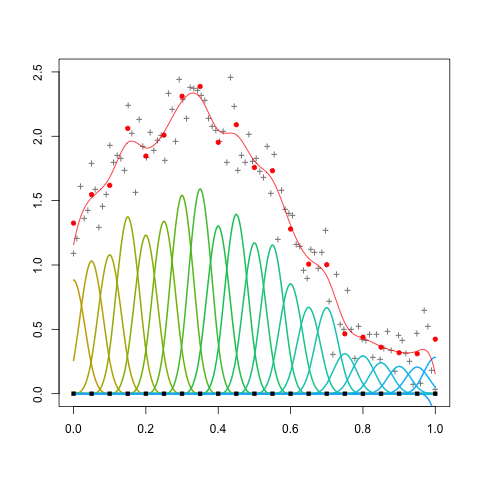
\includegraphics[scale=0.5]{pspline_pord2_xsmall_lambda.png}
  \label{fig:pspline_small_lambda}
\end{subfigure}
\begin{subfigure}{.5\textwidth}
  \centering
   \graphicspath{{img/}}
  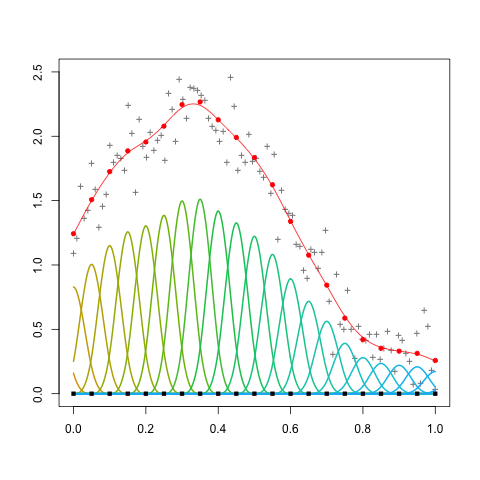
\includegraphics[scale=0.5]{pspline_pord2_small_lambda.png}
  \label{fig:pspline_small_lambda}
\end{subfigure}
\begin{subfigure}{.5\textwidth}
  \centering
   \graphicspath{{img/}}
  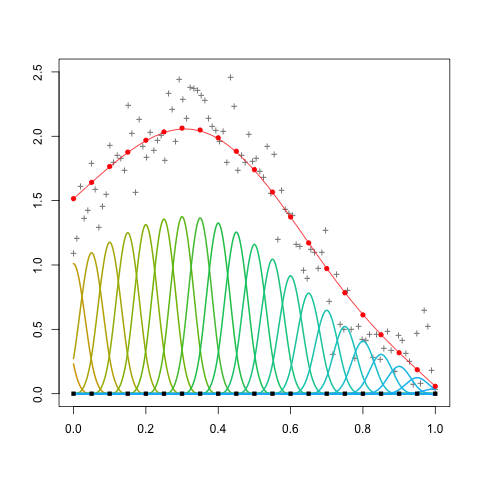
\includegraphics[scale=0.5]{pspline_pord2_medium_lambda.png}
  \label{fig:pspline_small_lambda}
\end{subfigure}
\begin{subfigure}{.5\textwidth}
  \centering
   \graphicspath{{img/}}
  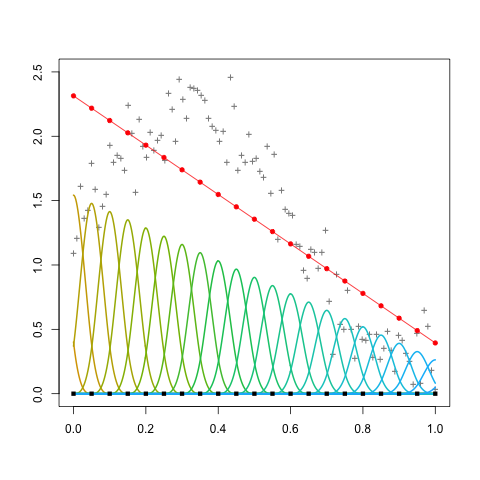
\includegraphics[scale=0.5]{pspline_pord2_large_lambda.png}
  \label{fig:pspline_small_lambda}
\end{subfigure}
\caption{\textit{Illustration of the impact of the second order difference penalty. The number of B-splines used is the same in each plot, with the value of the penalty parameter increasing from left to right and top to bottom across each plot. The fitted curve in the upper left plot is the most ``wiggly'' of any of the fits, as the penalty plays the weakest roll in the fitted coefficients there. The red circles are the values of each of the B-spline coefficients; as the penalty increases, they form as smoother sequence as we move across the four plots, which results in a smoother fitted function. As the penalty parameter approaches infinity, the fit approaches a linear function as shown in the bottom right plot.}}
\label{fig:second_ord_PS_pen_SML_lambda}
\end{figure}

The number of B-splines can be much larger than the number of observations because penalty ensures that the fitting procedure well-conditioned. One could literally use a thousand splines to fit ten observations without problems. Figure~\ref{fig:overcomplete_basis_pspline} illustrates this utility of the penalty for simulated data. There are $m=10$ data points and $K = 40 + 3$ cubic B-splines. This property of P-splines cannot be overly appreciated, as it allows us to completely circumvent the nontrivial task of the optimal selection of knot placement. But one simply cannot have too many B-splines. Unless computational constraints are of concern, which is possible with large models, it is prudent to use even more. 

\begin{figure}[H]   \label{fig:overcomplete_basis_pspline}
  \centering
   \graphicspath{{img/}}
  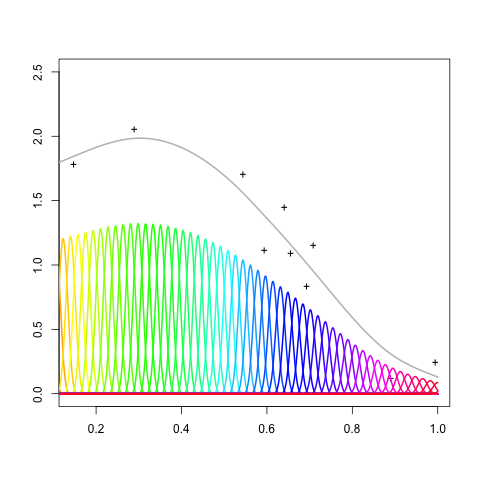
\includegraphics[scale=0.75]{pspline_10obs_60_basis_functions.png}
  \caption{P-spline smoothing of 10 observations using 60 B-spline basis functions.}
\end{figure}

%%====================================================================================

\subsection{Properties of P-splines}

P-splines enjoy many advantageous properties, many due in part to the inherited properties of the B-spline basis functions on which a generous portion of their foundation is constructed. 

\begin{enumerate}
\item \begin{description}\item[Boundary effects]
 P-splines show no boundary effects, as many types of kernel smoothers do. By this, we mean the spreading of a fitted curve or density outside of the (physical) domain of the data, generally accompanied by bending toward zero.
\end{description}
\item \begin{description}\item[P-splines fit polynomial data exactly.] 
P-splines can fit polynomial data exactly. Given data $\left(t_i,y_i\right)$, if the $y_i$ are a polynomial in $t$ of degree $k$, then B-splines of degree $k$ or higher will fit the data exactly. 
\begin{proof}
This statement is equivalent to the claim that given $\xi = \left\{ \xi_i \right\}$, $i=1,\dots,l+1$, and $g$ such that $y\left(t\right) = g\left(t\right)$, we can find an $f \in \PP_{k,\xi} \bigcap \mathscr{C}^{\left(k-2\right)}$ which agrees with $g$ at the points $\tau_1 < \dots < \tau_n$  with $\tau_i \in \left[\xi_1,\xi_{l+1}\right]$ for all $i$, where
\[
n=k+l-1
\]
The solution, $f$ is constructed as follows: generate the knot sequence $t = \left\{t_i\right\}$ as per the recipe in Theorem~\ref{curryschoenbergthm}:
\begin{align*}
t_1 &= t_2 = \dots = t_k = \xi_1 & \\
t_{k+i} &= \xi_{i+1}, & i=1,\dots,l-1\\
t_{n+1} &= t_{n+2} = \dots = t_{n+k} = \xi_{l+1} & 
\end{align*}

Let $\left\{ B_{ik} \right\}$, $i=1,\dots,n$ be the corresponding sequence of B-splines of order $k$, which are a basis for $\PP_{k,\xi} \bigcap \mathscr{C}^{\left(k-2\right)}$ by Theorem~\ref{curryschoenbergthm}. Here, $\PP_{k,\xi} \bigcap \mathscr{C}^{\left(k-2\right)}$ denotes the space of pp functions with breakpoints $\xi$ having two continuous (global) derivatives. Then, \cite{schoenberg1953polya} have shown that there exists exactly one $f \in \PP_{k,\xi} \bigcap \mathscr{C}^{\left(k-2\right)}$ agreeing with $g$ at $\tau_1,\dots, \tau_n$ if and only if 
\[
B_{ik}\left(\tau_i\right) \ne 0, \qquad \qquad i=1,\dots,n.
\]
This $f$ has a unique expansion of the form
\[
f = \sum_{i=1}^n a_i B_{ik}
\] 
for coefficients $a_i,\dots, a_n$, which are the solution to the linear system
\[
\sum_{j=1}^n a_jB_{jk}\left(\tau_i\right) = g\left(\tau_i\right), \qquad \qquad i=1,\dots,n.
\]
This system has a banded matrix of coefficients since $B_{jk}\left(\tau_i\right) \ne 0$ if and only if $\tau_i \in \left[t_j,t_{j+k}\right]$. So if $B_{jk}\left(\tau_i\right) \ne 0$ and thus $\tau_i \in \left(t_j,t_{j+k}\right)$, then there are at most $k$ of the $j$ indices such that $B_{jk}\left(\tau_i\right)$ is nonzero. And further, each of these indices $j$ must be such that 
\[
\left(t_i,t_{i+k}\right) \bigcap \left(t_j,t_{j+k}\right) \ne \emptyset,
\]
or such that $\vert i-j \vert < k$. At worst, the system corresponds to a banded matrix with $k-1$ lower and $k-1$ upper diagonals. 
\end{proof}
The same is true for P-splines if the order of the penalty is $k+1$ or higher, irrespective of the value of $\lambda$. Consider imposing a first-order difference penalty and a fit to data $y$ that is constant - a polynomial of degree 0. Since 
\[
\sum_{j=1}^n \hat{\alpha}_j B_j\left( x_i \right) = c, 
\]
\noindent
we have that
\[
\sum_{j=1}^n \hat{\alpha}_j B^\prime_j\left( x \right) = 0, 
\]
\noindent
for all $x$. From the relationship between differences and derivatives in \ref{eq:more_BS_properties} \ref{eq:BS_deriv_property}, 

\[
0 = \sum_{j=1}^n B^\prime_{j,k}\left(x\right) = \sum_{j=1}^n \Delta\alpha_{j+1} B_{j,k-1}\left( x \right), 
\]
\noindent
so that we must have $\Delta \alpha_j = 0$ for all $j$, and 
\[
\sum_{j=2}^n \Delta \alpha_j = 0.
\]

This shows that the penalty has no impact on the basis coefficients, and the resulting fit is identical to that when using unpenalized B-splines. Using induction, one can show that this is also true when the relationship between $x$ and $y$ is linear and a second order difference penalty is used, and for any values of the polynomial order and order of the difference penalty.\end{description}
\item \begin{description}\item[Null models under difference penalties]
The limiting P-spline fit approaches a polynomial under strongly enforced smoothing. As $\lambda \rightarrow \infty$, under a difference penalty of order $d$, the fitted function will approach a polynomial of degree $d-1$ as long as the degree of the B-splines is greater than or equal to $k$. To see this, we again need to use the relationship between the differenced coefficient sequence and the derivative of a B-spline as described in \ref{eq:more_BS_properties} \ref{eq:BS_deriv_property}. Consider using the second-order difference penalty; when $\lambda$ is large, the penalty dominates the P-spline objective function defined in \ref{eq:S_pen_varying_intercept_model}, so that the minimizer $\alpha$ must be such that $\sum_{j=3}^n\left(\Delta^2\alpha_j\right)^2$ is close to zero. Consequently, each of the individual second differences must also be nearly zero, and thus the second derivative of the fitted function must be close to zero over the entire domain.
\end{description}
\item \begin{description}\item[The limiting behaviour of $H_\lambda$] The trace of the hat matrix, 
\[
H_\lambda = B\left(B^TB + \lambda D_k^TD_k\right)^{-1}B^Ty
\] 
(or for $H$ defined for the addition of a varying slope component as in \ref{eq:simplest_VC_model_hat_matrix}) approaches $k$, the order of the differencing operator, as $\lambda$ increases. We index $H$ with the smoothing parameter to indicate that the elements of $H$ are a function of $\lambda$. Let
\begin{equation}
Q_B = B^T B \qquad \mbox{and} \qquad Q_\lambda = \lambda D^T D.
\end{equation}
Then using properties of the matrix trace, we can write
\begin{align}
\begin{split}
\mbox{tr}\left(H_\lambda \right) &= \mbox{tr}\bigg[ \left(Q_B + Q_\lambda \right)^{-1}Q_B \bigg]\\
&=\mbox{tr}\bigg[ Q_B^{1/2}\left(Q_B + Q_\lambda \right)^{-1}Q_B^{1/2} \bigg] \\
&=\mbox{tr}\bigg[\left(I + Q_B^{-{1/2}}Q_\lambda Q_B^{-{1/2}} \right)^{-1} \bigg]
\end{split}
\end{align}
Define $L \equiv Q_B^{-{1/2}}Q_\lambda Q_B^{-{1/2}}$. Then
\begin{equation}
\mbox{tr}\left(H_\lambda \right) = \mbox{tr}\bigg[\left(I + \lambda L \right)^{-1} \bigg] = \sum_{j=1}^n \frac{1}{1 + \lambda \gamma_j}
\end{equation}
 where $\gamma_j$, $j=1,\dots,n$ are the eigenvalues of $L$. $Q_\lambda$ has exactly $k$ eigenvalues equal to zero, hence $L$ has $k$ zero eigenvalues. For large $\lambda$, only the $k$ terms with $\gamma_j=0$ contribute to the sum which gives the trace of $H$, so that
 \[
\lim_{\lambda \rightarrow \infty  } \mbox{tr}\left(H\right) = k.
 \]
\end{description}
\end{enumerate}

The previous derivations hold regardless of whether we are fitting the varying intercept-only model, with $\mu\left( t\right) = \beta_0\left(t\right)$ or accommodating a varying slope for a regressor by specifying $\mu\left( t\right) = \beta_0\left(t\right) + \beta_1\left(t\right)x\left(t\right)$. The inspection of the hat matrix $H$ is a prelude to the following section, where we will discuss how to use the properties of $H$ to tune the smoothing parameter for optimal model selection. We will later show that extension of these results can be extended in a rather straightforward manner to the case that is of our particular interest: when the smooth slope function is a two-dimensional surface rather than a curve.


%%====================================================================================
%%====================================================================================


\subsection{Optimal tuning and model selection}

A major problem involved with any smoothing technique is the choice of the optimal amount of smoothing. We have illustrated how we can influence the smoothness of the estimated curve via $\lambda$, so we must now establish a way to choose the ``optimal'' value for it. Two potential model selection criteria are cross-validation and the Akaike information criterion, or AIC. In effect, AIC is an adjustment to the log likelihood to account for the effective dimension, or the effective number of parameters in the model. We choose to follow in the approach of\cite{eilers1996flexible}, \cite{marx2005multidimensional}, and \cite{buja1989linear} in using the trace of the smoother matrix as the effective dimension. This quantity is easily computed with the use of standard regression techniques, and is useful to compare the effective amount of smoothing for different numbers of knots, different degrees of the B-splines and different orders of penalties.

\subsubsection{Cross validation and information criteria}

\cite{hastie1986generalized} suggest using the trace of the smoother matrix as an approximation to the effective dimension, 

\subsubsection{P-splines as mixed models and the E-M algorithm}
%%====================================================================================
%%====================================================================================

\section{Tensor product B-splines for multidimensional surface approximation}

\begin{framed}
{ \needsparaphrased{ 
Loop the readers back to the original problem: estimating the $\phi\left(s,t \right) = \phi^*\left(l,m\right)$, which is the generalized autoregressive surface of interest when we model
\[
y\left(t\right) = \sum_{s < t} \phi\left(s,t\right) y\left(s\right) + \epsilon\left(t\right).
\] 
We need a way of extending the modeling framework discussed in the previous sections to multidimensional coefficient functions.
}  }
\end{framed}

\begin{framed}
{ \needsparaphrased{ 
Review the previously proposed methods of smoothing down the diagonals of the covariance matrix, including 
\begin{enumerate}
\item treating each diagonal as $p$ separate regression 
	\begin{enumerate}
	\item which does not permit one to model the smooth in the $s+t$ direction at all
	\item see \cite{huang2007estimation}
	\end{enumerate}
[\item Will I have already discussed Mohsen Pourahmadi's kernel smoothing technique at this point? If not, point out that kernel smoothing addresses the issue of the equally spaced observations as a necessity, but further elaborate that his method, failing to utilize the modified Cholesky decomposition, does not enjoy the unconstrained parameterization that we do; his methods do not ensure that covariance matrix estimates are positive definite. ]		
\item using GAMs to allow for each direction to have its own specified functional component
	\begin{enumerate}
	\item which only permits one to model the surface  as two smooth main effects: one in the $s-t$ directions and one in the $s+t$ direction. in the $s+t$ direction at all
	\end{enumerate} 
\end{enumerate}
}  }
\end{framed}

As in the previous chapter with smoothing splines, tensor products permit a nearly seamless extension of P-splines for VC models in which the slope function $\beta_1\left(\cdot\right)$ varies along a single indexing dimension to VC models with slope functions which are of two (or more) dimensions. If we equip each dimension, $x$ and $y$, with its own set of B-spline basis functions, then the only other modification necessary for the extension into two dimensions is the addition of a difference penalty for each augmented indexing variable.

Figure~\ref{fig:bicubic_BS} displays the building block of the foundation on which multidimensional P-splines is built: B-spline tensor product basis $\big\{ T_{jk}\big\}$.

\[
T_{jk}\left(x,y\right) = B_j\left(x\right)\bar{B}_k\left(y\right),
\]
where 
$\big\{ B_{j}\big\}$ and $\big\{ \bar{B}_{k}\big\}$ denote the B-spline bases for $x$ and $y$, having $n$ and $\bar{n}$ equally spaced knots along their respective domain.  


\begin{figure}[h]
\centering
 \graphicspath{{img/}}
  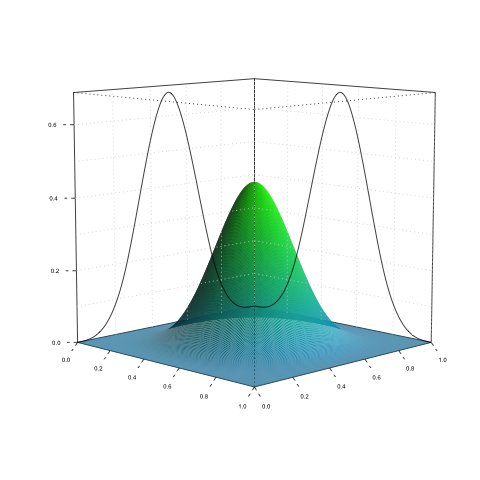
\includegraphics[width=4in, height=4in]{bicubic_basis_function.png}
 
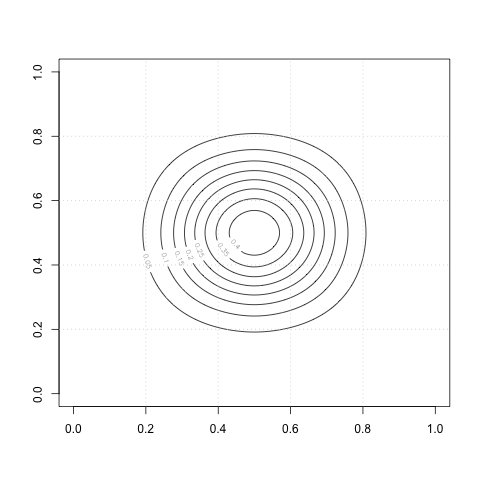
\includegraphics[width=4in, height=4in]{bicubic_bspline_contour.png}
\label{fig:bicubic_BS}
\caption{Tensor product of two cubic B-splines}
\end{figure}

\begin{figure}[H]
  \centering
  \graphicspath{{img/}}
  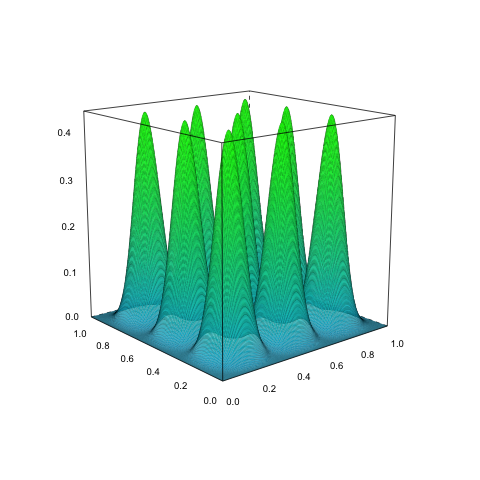
\includegraphics[width=5in,height=5in]{sparse_bicubic_basis.png}
  \caption{A subset of a full bivariate basis of cubic B-splines}\label{fig:sparse_bicubic_BS_basis}
\end{figure}


\end{document}